%%%%%%%%%%%%%%%%%%%%%%%%%%%%%%%%%%%%%%%%%%%%%%%%%%%%%%%%%%%%%%%%%%%%%%%%%%%%%%%%%%%%%%%%%%%%%%%%%%%%%%%%%%%%%%%%%%%%%%%%%%%%%%%%%%%%%%%%%%%%

%%%%%%%%%%%%%%%%%%%%%%%%%%%%%%%%%%%%%%%%%%%%%%%%%%%%%%%%%%%%%%   Author:Yao Zhang  %%%%%%%%%%%%%%%%%%%%%%%%%%%%%%%%%%%%%%%%%%%%%%%%%%%%%%%%%

%%%%%%%%%%%%%%%%%%%%%%%%%%%%%%%%%%%%%%%%%%%%%%%%%%%%%%%%%%  Email: jaafar_zhang@163.com  %%%%%%%%%%%%%%%%%%%%%%%%%%%%%%%%%%%%%%%%%%%%%%%%%%%%

%%%%%%%%%%%%%%%%%%%%%%%%%%%%%%%%%%%%%%%%%%%%%%%%%%%%%%%%%%%%%%%%%%%%%%%%%%%%%%%%%%%%%%%%%%%%%%%%%%%%%%%%%%%%%%%%%%%%%%%%%%%%%%%%%%%%%%%%%%%%%

\documentclass[aspectratio=2516]{beamer}
\mode<presentation> {
\usetheme{Madrid}
%\setbeamertemplate{footline} % To remove the footer line in all slides uncomment this line
}

\usepackage{graphicx} 
\graphicspath{ {img/} }
\usepackage[caption=false, font=footnotesize]{subfig}
\setbeamertemplate{caption}[numbered]
\newtheorem{rmk}{\kaishu 注释}
\newtheorem{defi}{\kaishu 定义}
\newtheorem{coro}{Corollary}
\newtheorem{thm}{\kaishu 定理}
\newtheorem{eg}{Example}
\newtheorem{proposition}{Proposition}
\newtheorem{lma}{Lemma}
\usepackage{algorithm}
\usepackage{algorithmic}
\renewcommand{\algorithmicrequire}{\textbf{Input:}}  
\renewcommand{\algorithmicensure}{\textbf{Output:}} 
\setbeamertemplate{theorems}[numbered]
\usepackage{bbding}
\usepackage{ctex}
\renewcommand{\figurename}{Figure}
\renewcommand{\tablename}{Table}
\renewcommand{\proofname}{\kaishu 证明}

%-----------------------------------------------------------------------------------------------------------------------------------------------
\title[ \kaishu 向量分析之应用]{ \kaishu 向量分析之应用} 
\vspace{4.5cm}

\author{Yao Zhang} 

\institute[UCAS \& NAOC] 
{	
    
    \kaishu 
    
    University of Chinese Academy of Sciences 
    
    \vspace{0.2cm}
    
    National Astronomical Observatories, Chinese Academy of Sciences 
     
	 \vspace{0.5cm}
	 
	 {\color{blue} 特别说明: 投影片主要基于林琦焜老师所写的 <<向量分析>> {\tiny \cite{p1}}.} 
	 
	 \vspace{0.5cm}
	
	{\tiny 讲义电子版见: {\color{blue} \url{https://zhims.github.io/doc/note/analysis/VectorAnalysis/chapter5.pdf}}}
}

\date{ \kaishu \today }


\logo{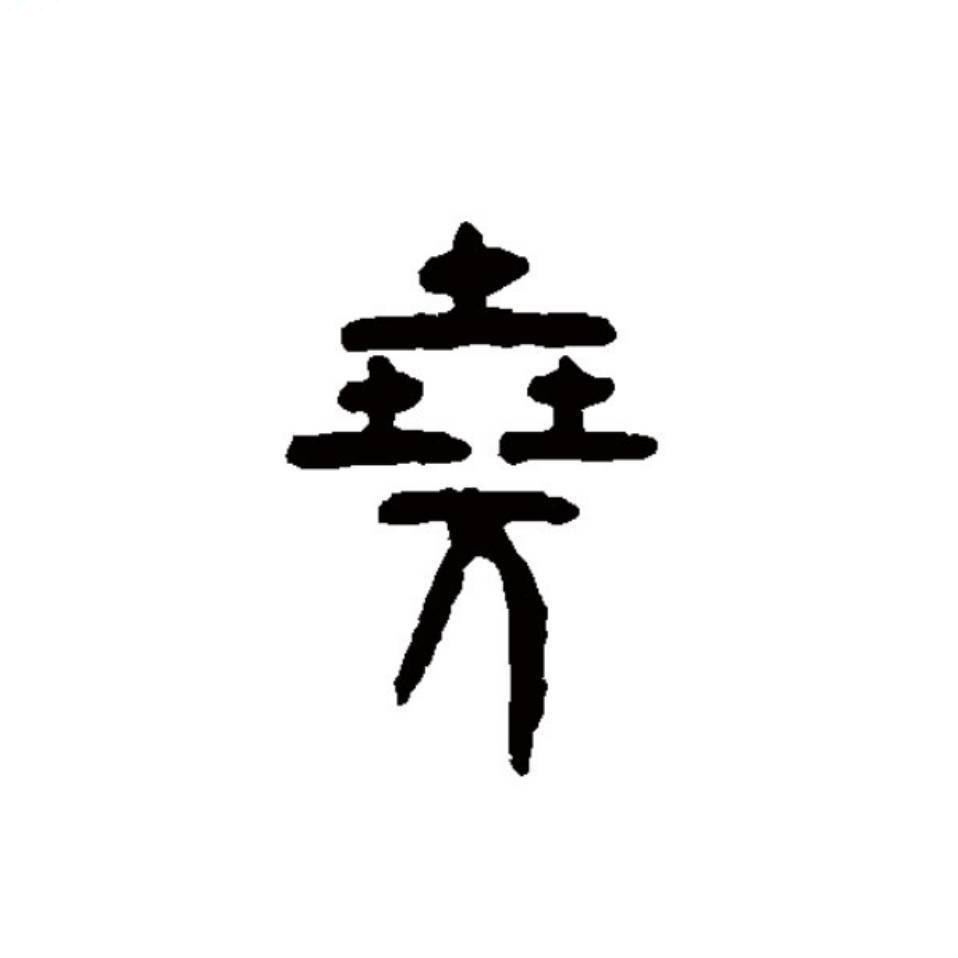
\includegraphics[height=0.6cm]{yao.jpg}}

%------------------------------------------------------------------------------------------------------------------------------------------

\begin{document}
	\begin{frame}
	\titlepage 
	\end{frame}

%-------------------------------------------------------------------------------------------------------------------------------------------


\begin{frame}
\frametitle{\kaishu 向量分析之意义}

\kaishu 

\vspace{-0.25cm}

{\color{blue} 数学家们可以怀疑他们得到的结果是否适用于立体几何学,流体静力学或电磁学. 但是, 正如我们现在所研究的自然哲学一样, 必然赋予我们的运算以某种形式, 对其每一步骤必须能够作出物理学的解释. 在这里, 我们的计算能力比较纯粹的计算原则的运用和对结果的解释更有用处. 
	
	--- James Clerk Maxwell, 1831-1879}

\vspace{0.35cm}

正如微积分是为了解决牛顿力学自然而然发展出来的一门学问, 向量分析也是因为想要了解电磁学而应运而生的一门学问, 任何一门有活力的数学必定是为了解决问题而来.

\vspace{0.35cm}

{\color{blue} 任何科学只要能产生充裕的问题, 就有丰富的生命力, 若问题匮乏, 就显示了死亡或发展停顿. 
	
	--- David Hilbert, 1862-1943}

\end{frame}

%--------------------------------------------------------------------------------------------------------------------------------------------

\begin{frame}
\frametitle{\kaishu 主要内容} 
\begin{small}
	\tableofcontents
\end{small} 
\end{frame}

%--------------------------------------------------------------------------------------------------------------------------------------------


%----------------------------- section 1 ----------------------------------------------------------------------------------------------------

\section{\kaishu 流体力学之 Euler 方程方式}

%--------------------------------------------------------------------------------------------------------------------------------------------

\begin{frame}
\frametitle{\kaishu 第  \uppercase\expandafter{\romannumeral1} 节}
\begin{center}
	\Large \kaishu 流体力学之 Euler 方程方式
\end{center}
\end{frame}

%--------------------------------------------------------------------------------------------------------------------------------------------

\begin{frame}
\frametitle{\kaishu 质量守恒定律}

\kaishu 

物理学有一些基本定律, 其中之一就是质量守恒定律(conservation of mass). 利用微分方程可以讲这定律用数学的式子表达出来, 透过方程式以精确的数学理论来研究可以帮助我们理解大自然并探索宇宙的奥妙. Euler 方程是由质量守恒与动量守恒, 还有能量守恒三大定律所组成. 我们先考虑无黏性的理想气体: 空间任意一区域 $ V $, 假设其密度为 $\rho \left( {\boldsymbol{x},t} \right)$, 其质量等于

\begin{equation}
M\left( t \right) = \iiint_V {\rho \left( {\boldsymbol{x},t} \right)dV} \qquad  (\text{\kaishu 质量 $ = $ 密度 $ \times $  体积})
\label{eq5.1.1}
\end{equation}

\vspace{0.15cm}

质量的变化等于质量对时间 $ t $ 的微分

\begin{equation}
\frac{{dM\left( t \right)}}{{dt}} = \iiint_V {\frac{{\partial \rho  (\boldsymbol{x},t)}}{{\partial t}}dV}
\label{eq5.1.2}
\end{equation}

\end{frame}

%--------------------------------------------------------------------------------------------------------------------------------------------

\begin{frame}
\frametitle{\kaishu 质量守恒定律}

\kaishu 

另一方面我们可以计算从 $ V $ 的表面 $ \partial V = S$ 进出的质量得出质量的变率. 假设流体的速度是 $u\left( {\boldsymbol{x},t} \right)$ 则单位时间 $ dt $ 内流体移动的距离(长度)为  {\color{red} $ \boldsymbol{u} \times  dt $} 而高则为(投影) $ dt \ \boldsymbol{u}\cos \left(\boldsymbol{x}, \boldsymbol{n}\right) $ 其 $ \boldsymbol{n} $ 为法向量, 所以体积等于

\begin{equation}
\boldsymbol{u}\cos \left( {\boldsymbol{u},\boldsymbol{n}} \right)dtdS \qquad (\text{\kaishu 高 $ \times $ 底面积})
\end{equation}

其中 $ \cos \left( {\boldsymbol{u},\boldsymbol{n}} \right) $ 是 $ \boldsymbol{u},\boldsymbol{n} $ 的方向余弦. 此时的质量等于

\begin{equation}
\rho \boldsymbol{u}\cos \left( {\boldsymbol{u},\boldsymbol{n}} \right)dtdS \qquad (\text{\kaishu 密度 $ \times $ 体积})
\notag 
\end{equation}

沿着表面积分(曲面积分) 可得全部得质量

\begin{equation}
\iint_S {\rho \boldsymbol{u}\cos \left( {\boldsymbol{u},\boldsymbol{n}} \right)dtdS}
\label{eq5.1.4}
\end{equation}

这是时间 $ dt $ 内得质量, 所以外流的速度率(通量)为(除以 $ dt $)

\begin{equation}
\iint_S {\rho \boldsymbol{u}\cos \left( {\boldsymbol{u},\boldsymbol{n}} \right)dS} = \iint_S {\rho \boldsymbol{u} \cdot \boldsymbol{n}dS}
\notag 
\end{equation}

\end{frame}

%--------------------------------------------------------------------------------------------------------------------------------------------

%--------------------------------------------------------------------------------------------------------------------------------------------

\begin{frame}
\frametitle{\kaishu 质量守恒定律}

\kaishu 

根据质量不灭(守恒)定律: 一物质的质量变化和该物质进出表面的改变(通量)是一样的. 因此

\vspace{0.15cm}

\begin{equation}
\iiint_V {\frac{{\partial \rho }}{{\partial t}}dV} =  - \iint_S {\rho \boldsymbol{u} \cdot \boldsymbol{n}dS}
\label{eq5.1.5}
\end{equation}

\vspace{0.15cm}

上面这个方程式右式的曲面积分可以运用散度定理转化成体积分(volume integral)

\vspace{0.15cm}

\begin{equation}
\iint_S {\rho \boldsymbol{u} \cdot \boldsymbol{n}dS} = \iiint_V {\nabla  \cdot \left( {\rho \boldsymbol{u}} \right)dV}
\notag
\end{equation}

\vspace{0.15cm}

因此

\vspace{0.15cm}

\begin{equation}
\iiint_V {\frac{{\partial \rho }}{{\partial t}} + \nabla  \cdot \left( {\rho \boldsymbol{u}} \right)dV} = 0
\label{eq5.1.6}
\end{equation}

\end{frame}

%--------------------------------------------------------------------------------------------------------------------------------------------

%--------------------------------------------------------------------------------------------------------------------------------------------

\begin{frame}
\frametitle{\kaishu 质量守恒定律}

\kaishu 

由于我们考虑的是任意的区域 $ V $, 因此可以将 $ V $ 缩成只有一点再利用连续特质可结论: 被积分函数必定是 0

\vspace{0.5cm}

\begin{equation}
\frac{{\partial \rho }}{{\partial t}} + \nabla  \cdot \left( {\rho \boldsymbol{u}} \right) = 0
\label{eq5.1.7}
\end{equation}

\vspace{0.5cm}

或 $\boldsymbol{u} = \left( {u,v,w} \right)$

\begin{equation}
\frac{{\partial \rho }}{{\partial t}} + \frac{\partial }{{\partial x}}\left( {\rho u} \right) + \frac{\partial }{{\partial y}}\left( {\rho v} \right) + \frac{\partial }{{\partial z}}\left( {\rho w} \right) = 0
\label{eq5.1.8}
\end{equation}

\vspace{0.5cm}

这个微分方程 \ref{eq5.1.7} 或 \ref{eq5.1.8} 称为连续方程(continuity equation). 它就是质量守恒律: 流体沿别界 $\partial V = S$ 的流量多寡(通量)等于全部质量随时间的该变量. 

\end{frame}

%--------------------------------------------------------------------------------------------------------------------------------------------

\begin{frame}
\frametitle{\kaishu 动量守恒律}

\kaishu 

其次我们推导动量守恒律(conservation of momentum), 压力 $ P $ 作用到边界 $\partial V = S$ 水平方向 $ x $ 轴的力等于:

\vspace{0.1cm}

\begin{equation}
- \iint_S {Pdydz} =  - \iiint_V {\frac{{\partial P}}{{\partial x}}dV} \qquad (\text{\color{cyan} \kaishu 力 = 压力 $ \times $ 面积 })
\label{eq5.19}
\end{equation}

\vspace{0.1cm}

另外位置向量为 $\boldsymbol{r} = \left( {x,y,z} \right) = \left( {x\left( t \right),y\left( t \right),z\left( t \right)} \right)$, 所以 $ x- $方向速度 $\mathop x\limits^ \cdot   = u$, 而 $ x- $方向加速度为 $\mathop x\limits^{ \cdot  \cdot }  = \mathop u\limits^ \cdot  $, 整体的加速度等于

\vspace{0.1cm}

\begin{equation}
\frac{{du}}{{dt}} = \frac{{\partial u}}{{\partial t}} + u\frac{{\partial u}}{{\partial x}} + v\frac{{\partial u}}{{\partial y}} + w\frac{{\partial u}}{{\partial z}} = \frac{{\partial u}}{{\partial t}} + \left( {\boldsymbol{u} \cdot \nabla } \right)u
\label{eq5.1.10}
\end{equation}

\vspace{0.1cm}

由牛顿第二运动定律 $ F = ma $, 可得

\vspace{0.1cm}

\begin{equation}
\frac{{du}}{{dt}} = \mathop {\lim }\limits_{\left| V \right| \to 0} \left( {\frac{{ - \iiint_V {\frac{{\partial P}}{{\partial x}}dV}}}{{\iiint_V {\rho dV}}}} \right)
\label{eq5.11}
\end{equation}

\end{frame}

%--------------------------------------------------------------------------------------------------------------------------------------------

%--------------------------------------------------------------------------------------------------------------------------------------------

\begin{frame}
\frametitle{\kaishu 动量守恒律}

\kaishu 

再次利用连续性:

\begin{equation}
\frac{{\partial u}}{{\partial t}} + u\frac{{\partial u}}{{\partial x}} + v\frac{{\partial u}}{{\partial y}} + w\frac{{\partial u}}{{\partial z}} + \frac{1}{\rho }\frac{{\partial P}}{{\partial x}} = 0
\label{eq5.1.12}
\end{equation}

同理如果考虑 $ y,z $ 方向:

\begin{equation}
\frac{{\partial v}}{{\partial t}} + u\frac{{\partial v}}{{\partial x}} + v\frac{{\partial v}}{{\partial y}} + w\frac{{\partial v}}{{\partial z}} + \frac{1}{\rho }\frac{{\partial P}}{{\partial y}} = 0
\label{eq5.1.13}
\end{equation}

\begin{equation}
\frac{{\partial w}}{{\partial t}} + u\frac{{\partial w}}{{\partial x}} + v\frac{{\partial w}}{{\partial y}} + w\frac{{\partial w}}{{\partial z}} + \frac{1}{\rho }\frac{{\partial P}}{{\partial z}} = 0
\label{eq5.1.14}
\end{equation}

或者将 \ref{eq5.1.12} -- \ref{eq5.1.14} 写成向量的形式:

\begin{equation}
{\partial _t}\boldsymbol{u} + \left( {\boldsymbol{u} \cdot \nabla } \right)\boldsymbol{u} + \frac{1}{\rho }\nabla P = 0
\label{eq5.1.15}
\end{equation}

这就是动量守恒律, 它本质上就是牛顿第二运动定律.
\end{frame}

%--------------------------------------------------------------------------------------------------------------------------------------------

\begin{frame}
\frametitle{\kaishu 可压缩 Euler 方程}

\vspace{-0.25cm}

\begin{defi}[\kaishu 可压缩 Euler 方程]
	\kaishu 
	假设压力只与密度有关 $P = P\left( \rho  \right)$
	
	\begin{equation}
	\frac{{\partial \rho }}{{\partial t}}   + \nabla  \cdot \left( {\rho \boldsymbol{u}} \right)  = 0
	\notag 
	\end{equation}
	\vspace{-0.5cm}
	\begin{equation}
	{\partial _t}\boldsymbol{u} +  \left( {\boldsymbol{u} \cdot \nabla } \right)\boldsymbol{u} + \frac{1}{\rho }\nabla P  = 0
	\notag 
	\end{equation}
	
	如果有外力项 $ \boldsymbol{f} $ 则为
	
	\begin{equation}
	\frac{{\partial \rho }}{{\partial t}}   + \nabla  \cdot \left( {\rho \boldsymbol{u}} \right)  = 0
	\label{eq5.1.16}
	\end{equation}
	
	\begin{equation}
	{\partial _t}\boldsymbol{u} + \left( {\boldsymbol{u} \cdot \nabla } \right)\boldsymbol{u} + \frac{1}{\rho }\nabla P = \frac{\boldsymbol{f}}{\rho }
	\label{eq5.1.17}
	\end{equation}
\end{defi}
\end{frame}

%--------------------------------------------------------------------------------------------------------------------------------------------

\begin{frame}
\frametitle{\kaishu 可压缩 Euler 方程之注解}

\kaishu 

\small 

\begin{enumerate}
	\item \small  任何一个有物理意义的方程必须满足量纲平衡(dimensional balance) 之要求, 质量守恒律 \ref{eq5.1.7}:
	\begin{equation}
	\left[ {\frac{{\partial \rho }}{{\partial t}}} \right] \approx \left[ {\nabla  \cdot \left( {\rho {\boldsymbol{u}}} \right)} \right] \Rightarrow \frac{1}{T}\frac{M}{{{L^3}}} = \frac{1}{L}\frac{M}{{{L^3}}}\frac{L}{T}
	\notag 
	\end{equation}
	\item \small 动量守恒律 \ref{eq5.1.17}:
	\begin{equation}
	\left[ {{\partial _t}\boldsymbol{u}} \right] \approx \left[ {\left( {\boldsymbol{u} \cdot \nabla } \right)\boldsymbol{u}} \right] \approx \left[ {\frac{1}{\rho }\nabla P} \right] \approx \left[ {\frac{\boldsymbol{f}}{\rho }} \right]
	\notag 
	\end{equation}
	\begin{equation}
	\frac{1}{T}\frac{L}{T} = \frac{L}{T}\frac{1}{L}\frac{L}{T} = \frac{1}{{{M \mathord{\left/
					{\vphantom {M {{L^3}}}} \right.
					\kern-\nulldelimiterspace} {{L^3}}}}}\frac{1}{L}\frac{{{{ML} \mathord{\left/
					{\vphantom {{ML} {{T^2}}}} \right.
					\kern-\nulldelimiterspace} {{T^2}}}}}{{{L^2}}} = \frac{{{{ML} \mathord{\left/
					{\vphantom {{ML} {{T^2}}}} \right.
					\kern-\nulldelimiterspace} {{T^2}}}}}{{{M \mathord{\left/
					{\vphantom {M {{L^3}}}} \right.
					\kern-\nulldelimiterspace} {{L^3}}}}}
	\notag 
	\end{equation}
	这里我们用到关系式 $P = {F \mathord{\left/
			{\vphantom {F A}} \right.
			\kern-\nulldelimiterspace} A},\;F = ma$, 因此若 $ P $ 是压力({\color{red} 压强}),  $ \boldsymbol{f} $ 代表力则 \ref{eq5.1.7} 的第三项,第四项必定含有 $\frac{1}{\rho }$ 这一项.
	\item \small 利用连续方程 \ref{eq5.1.7},\ref{eq5.1.15}, \ref{eq5.1.17} 可以改写为
	\begin{equation}
	\color{red}
	{\partial _t}\left( {\rho \boldsymbol{u}} \right) + div\left( {\rho \boldsymbol{u} \otimes \boldsymbol{u}} \right) + \nabla P = 0 \quad  {\partial _t}\left( {\rho \boldsymbol{u}} \right) + div\left( {\rho \boldsymbol{u} \otimes \boldsymbol{u}} \right) + \nabla P = \boldsymbol{f}
	\notag 
	\end{equation}
	
\end{enumerate}

\end{frame}

%--------------------------------------------------------------------------------------------------------------------------------------------

\begin{frame}
\frametitle{\kaishu Navier-Stokes 方程}

\kaishu 

如果将黏性(viscosity)也考虑进来就是著名的 Navier-Stokes 方程

\vspace{0.75cm}

\begin{defi}[\kaishu 可压缩 Navier-Stokes 方程]
	
	\kaishu 
	
	$ P = P(\rho) $,
	\begin{equation}
	\frac{{\partial \rho }}{{\partial t}} + \nabla  \cdot \left( {\rho \boldsymbol{u}} \right) = 0
	\label{eq5.1.18}
	\end{equation}
	
	\vspace{0.25cm}
	
	\begin{equation}
	{\partial _t}\boldsymbol{u} + \left( {\boldsymbol{u} \cdot \nabla } \right)\boldsymbol{u} + \frac{1}{\rho }\nabla P = \nu \Delta \boldsymbol{u} + \frac{\boldsymbol{f}}{\rho }
	\label{eq5.1.19}
	\end{equation}
	
	\vspace{0.25cm}
	
	根据量纲平衡之要求, 黏性系数 $ \nu  $ 必须带有量纲 $\left[ v \right] = \frac{{{L^2}}}{T}$. 
\end{defi}

\end{frame}

%--------------------------------------------------------------------------------------------------------------------------------------------

\begin{frame}
\frametitle{\kaishu 能量守恒定律}

\kaishu 

\begin{defi}[\kaishu 随物导数]
	
	\kaishu 
	
	我们称
	\begin{equation}
	\frac{D}{{Dt}} = \frac{\partial }{{\partial t}} + \boldsymbol{u} \cdot \nabla  = \frac{\partial }{{\partial t}} + u\frac{\partial }{{\partial x}} + v\frac{\partial }{{\partial y}} + w\frac{\partial }{{\partial z}}
	\label{eq5.1.20}
	\end{equation}
	这个算子为随物导数(material derivative), 它表示当我们随着一个流体观测它性质的变化率.
\end{defi}

\end{frame}

%--------------------------------------------------------------------------------------------------------------------------------------------

\begin{frame}
\frametitle{\kaishu 能量守恒定律}

\kaishu 

\small 
 
要推导能量守恒律, 必须引进热力学的概念. 其中常见的有熵(entropy) S, 比热(ratio of specific heat) $ \gamma $, $ \gamma > 1 $. 此时压力({\color{red} 压强}),熵与密度之关系为:

\begin{equation}
\tiny 
P(\rho, S) = A(S) \rho^{\gamma}
\label{eq5.1.21}
\end{equation}

则能量守恒律其实就是熵沿粒子路径(particle path) 都是固定数的常数, 即:

\begin{equation}
\tiny 
\frac{{DS}}{{Dt}} = \frac{{\partial S}}{{\partial t}} + u\frac{{\partial S}}{{\partial x}} + v\frac{{\partial S}}{{\partial y}} + w\frac{{\partial S}}{{\partial z}} = \left( {\frac{\partial }{{\partial t}} + \boldsymbol{u} \cdot \nabla } \right)S = 0
\label{eq5.1.22}
\end{equation}

也就是说当我们跟定一个流体粒子时它的熵是不变的.

\vspace{0.15cm}

利用 \ref{eq5.1.21},\ref{eq5.1.22} 式也可以改写为:

\begin{equation}
\tiny
\frac{\partial }{{\partial t}}\left( {\frac{P}{{{\rho ^\gamma }}}} \right) + u\frac{\partial }{{\partial x}}\left( {\frac{P}{{{\rho ^\gamma }}}} \right) + v\frac{\partial }{{\partial y}}\left( {\frac{P}{{{\rho ^\gamma }}}} \right) + w\frac{\partial }{{\partial z}}\left( {\frac{P}{{{\rho ^\gamma }}}} \right) = 0
\label{eq5.1.23}
\end{equation}

\begin{equation}
\tiny
\frac{D}{{Dt}}\left( {\frac{P}{{{\rho ^\gamma }}}} \right) = \frac{\partial }{{\partial t}}\left( {\frac{P}{{{\rho ^\gamma }}}} \right) + \left( {\boldsymbol{u} \cdot \nabla } \right)\left( {\frac{P}{{{\rho ^\gamma }}}} \right) = 0
\label{eq5.1.24}
\end{equation}

\end{frame}

%--------------------------------------------------------------------------------------------------------------------------------------------

\begin{frame}
\frametitle{\kaishu 声学方程式}

\kaishu 

代入 Euler 方程(我们承认 $ (\boldsymbol{u}, \rho, P(\rho)) $ 是 Euler 方程的解) 并忽略高阶项可得声学方程式 (Acoustic equation).

\vspace{0.15cm}

\begin{thm}[\kaishu 声学方程式]
	\begin{equation}
	\color{red}
	\frac{{\partial {\rho _1}}}{{\partial t}} + {\rho _0}div\;{\boldsymbol{u}_1} = 0
	\label{eq5.1.26}
	\end{equation}

\vspace{0.15cm}	
	
	\begin{equation}
	\color{red}
	\frac{{\partial {\boldsymbol{u}_1}}}{{\partial t}} + \frac{{P^{\prime}\left( {{\rho _0}} \right)}}{{{\rho _0}}}\nabla {\rho _1} = 0
	\label{eq5.1.27}
	\end{equation}
\end{thm}

\end{frame}

%--------------------------------------------------------------------------------------------------------------------------------------------

\begin{frame}
\frametitle{\kaishu 声学方程式之注解}

\kaishu 

\small 

\begin{enumerate}
	\item 声学方程式 \ref{eq5.1.26}, \ref{eq5.1.27} 也称为 Euler 方程之线性化(linearization). 这是研究非线性方程的最基本方法.
	\item 声学方程式 \ref{eq5.1.26}, \ref{eq5.1.27} 消去速度 $ \boldsymbol{u}_{1} $ 则密度 $ \rho_1 $ 满足波动方程
	\begin{equation}
	\tiny
	\frac{{{\partial ^2}{\rho _1}}}{{\partial {t^2}}} = {P^{\prime}}\left( {{\rho _0}} \right)\Delta {\rho _1} \equiv {c^2}\Delta {\rho _1}
	\label{eq5.1.28}
	\end{equation}
	$c = \sqrt {{P^{\prime}}\left( {{\rho _0}} \right)} $ 是声速(sound speed). 为什么 $c = \sqrt {{P^{\prime}}\left( {{\rho _0}} \right)} $  是声速? 籍由量纲分析
	\begin{equation}
	\tiny 
	{\left[ c \right]^2} = \left[ {{P^{\prime}}\left( {{\rho _0}} \right)} \right] = \frac{{\left[ P \right]}}{{\left[ {{\rho _0}} \right]}} = \frac{{{M \mathord{\left/
					{\vphantom {M {L{T^2}}}} \right.
					\kern-\nulldelimiterspace} {L{T^2}}}}}{{{M \mathord{\left/
					{\vphantom {M {{L^3}}}} \right.
					\kern-\nulldelimiterspace} {{L^3}}}}} = \frac{{{L^2}}}{{{T^2}}}
	\notag
	\end{equation}
	$ c $ 之量纲(dimension) 正是速度! 压力({\color{red} 压强}) 对密度的微分是声速的平方. 
	\item 波动方程 \ref{eq5.1.28} 是线性而压力 $P = P\left( {{\rho _0}} \right)$ 是密度 $ \rho_0 $ 的函数因此则压力 $ P $ 也满足相同的波动方程
	\begin{equation}
	\tiny 
	\frac{{{\partial ^2}P}}{{\partial {t^2}}} = {c^2}\Delta P
	\label{eq5.1.29}
	\end{equation}

\end{enumerate}

\end{frame}

%--------------------------------------------------------------------------------------------------------------------------------------------

\begin{frame}
\frametitle{\kaishu 声学方程式之注解}

\kaishu 

\begin{enumerate}
	
	\setcounter{enumi}{3}

	\item 如果假设 $\nabla  \times {\boldsymbol{u}_1} = 0$ 则
	\begin{equation}
	\nabla div\;{\boldsymbol{u}_1}\; = \Delta {\boldsymbol{u}_1} + \nabla  \times \left( {\nabla  \times {\boldsymbol{u}_1}} \right) = \Delta {\boldsymbol{u}_1}
	\notag 
	\end{equation}
	消去密度 $ \rho_1 $ 则速度 $ \boldsymbol{u}_{1} $ 也满足波动方程
	
	\begin{equation}
	\frac{{{\partial ^2}{\boldsymbol{u}_1}}}{{\partial {t^2}}} = {c^2}\Delta {\boldsymbol{u}_1}
	\label{eq5.1.30}
	\end{equation}
	
	若引进速度位 $ U $, $\nabla U = {\boldsymbol{u}_1}$ 则 $ U $ 也满足相同的波动方程
	
	\begin{equation}
	\frac{{{\partial ^2}U}}{{\partial {t^2}}} = {c^2}\Delta U
	\label{eq5.1.31}
	\end{equation}
	
	因此声学方程式中的密度 $ \rho_1 $, 压力 $ P_{1} $, 速度 $ \boldsymbol{u}_{1} $ 与速度位 $ U $ 都满足相同的波动方程且以相同的速率 $ \pm c$ 传递.
\end{enumerate}

\end{frame}

%--------------------------------------------------------------------------------------------------------------------------------------------


%----------------------------- section 2 ----------------------------------------------------------------------------------------------------

\section{\kaishu  不可压缩流体}

%--------------------------------------------------------------------------------------------------------------------------------------------

\begin{frame}
\frametitle{ \kaishu 第 \uppercase\expandafter{\romannumeral2} 节}
\begin{center}
	\Large \kaishu  不可压缩流体
\end{center}
\end{frame}

%-------------------------------------------------------------------------------------------------------------------------------------------

\begin{frame}
\frametitle{\kaishu 不可压缩流体}

\kaishu 

\small

有了速度的概念之后, 我们觉得这是很好的时机来阐释散度(divergence) 的物理意义, 我们可以这么想象: 假设正在喝咖啡将奶精倒入杯内, 最初形成的图形为 $ \Omega_{0} $, 而后经由搅拌或其他因素使得$ \Omega_{0} $ 变化, 其位置向量为 $\left( {x\left( t \right),y\left( t \right)} \right) = \left( {\xi ,\eta } \right)$, 速度则为 $ \boldsymbol{u}\left(t\right)  = \left( {\frac{{dx}}{{dt}},\frac{{dy}}{{dt}}} \right) = \left( {u,v} \right)$, 经过 $ t $ 时间之后 $ \Omega_{0} $ 转换为 $ \Omega_{t} $, 我们有兴趣的问题是 $ \Omega_{0} $ 与 $ \Omega_{t} $, 两者之面积变化为何? (实际上牛顿力学本身就是一种坐标变换) 我们看其中一小块($d{V_0} \to d{V_t}$) 两者关系为

\begin{equation}
\tiny 
d{V_0} = dxdy = \frac{{\partial \left( {x,y} \right)}}{{\partial \left( {\xi ,\eta } \right)}} = J\left( t \right)d\xi d\eta  = J\left( t \right)d{V_t}
\label{eq5.2.1}
\end{equation}

其中 $J\left( t \right)$ 就是 Jacobian

\begin{equation}
\tiny 
J\left( t \right) = \left| {\frac{{\partial \left( {x,y} \right)}}{{\partial \left( {\xi ,\eta } \right)}}} \right| = \left| {\begin{matrix}
	{\frac{{\partial x}}{{\partial \xi }}} & {\frac{{\partial x}}{{\partial \eta }}}  \\ 
	{\frac{{\partial y}}{{\partial \xi }}} & {\frac{{\partial y}}{{\partial \eta }}}  \\ 
	\end{matrix} } \right| = \frac{{d{V_0}}}{{d{V_t}}}
\label{eq5.2.2}
\end{equation}

\begin{figure}[!htb]
	\centering
	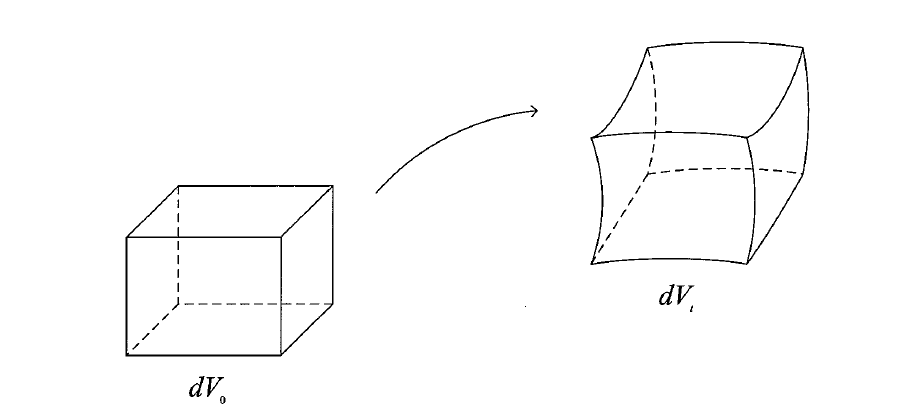
\includegraphics[width=0.35\linewidth,height=0.15\linewidth]{/ch5/fig_5_2_1.png}
	\label{img001}
	%\caption{}
\end{figure}

\end{frame}

%-------------------------------------------------------------------------------------------------------------------------------------------

\begin{frame}
\frametitle{\kaishu 不可压缩流体}

\kaishu 

\small

因此 ${\Omega _0} \to {\Omega _t}$ 之变化情形, 等于是探讨 $ J\left(t\right) $ 的变化, 我们假设 $ J,J^{-1} \ne 0 $, 即没有退化的情形(可设 $ 0 < J < \infty $ ): 由全微分(total differential) 知:

\begin{equation}
\frac{d}{{dt}}\left( {\frac{{\partial x}}{{\partial \xi }}} \right) = \frac{\partial }{{\partial \xi }}\left( {\frac{{dx}}{{dt}}} \right) = \frac{{\partial u}}{{\partial \xi }} = \frac{{\partial u}}{{\partial x}}\frac{{\partial x}}{{\partial \xi }} + \frac{{\partial u}}{{\partial y}}\frac{{\partial y}}{{\partial \xi }}
\notag 
\end{equation}

同理可得

\begin{equation}
\begin{split}
\frac{d}{{dt}}\left( {\frac{{\partial x}}{{\partial \eta }}} \right) & = \frac{{\partial u}}{{\partial x}}\frac{{\partial x}}{{\partial \eta }} + \frac{{\partial u}}{{\partial y}}\frac{{\partial y}}{{\partial \eta }}\\
\frac{d}{{dt}}\left( {\frac{{\partial y}}{{\partial \xi }}} \right) & = \frac{{\partial u}}{{\partial x}}\frac{{\partial x}}{{\partial \xi }} + \frac{{\partial u}}{{\partial y}}\frac{{\partial y}}{{\partial \xi }} \\
\frac{d}{{dt}}\left( {\frac{{\partial y}}{{\partial \eta }}} \right) & = \frac{{\partial u}}{{\partial x}}\frac{{\partial x}}{{\partial \eta }} + \frac{{\partial u}}{{\partial y}}\frac{{\partial y}}{{\partial \eta }}
\end{split}
\notag 
\end{equation}

\end{frame}

%-------------------------------------------------------------------------------------------------------------------------------------------

\begin{frame}
\frametitle{\kaishu 不可压缩流体}

\kaishu 

\small

$ J\left(t\right) $ 对 $ t $ 微分并利用行列式之性质可得
\begin{equation}
\tiny 
\begin{split}
	\frac{{dJ}}{{dt}} & = \left| {\begin{matrix}
		{\frac{d}{{dt}}\frac{{\partial x}}{{\partial \xi }}} & {\frac{d}{{dt}}\frac{{\partial x}}{{\partial \eta }}}  \\ 
		{\frac{{\partial y}}{{\partial \xi }}} & {\frac{{\partial y}}{{\partial \eta }}}  \\ 
		\end{matrix} } \right| + \left| {\begin{matrix}
		{\frac{{\partial x}}{{\partial \xi }}} & {\frac{{\partial x}}{{\partial \eta }}}  \\ 
		{\frac{d}{{dt}}\frac{{\partial y}}{{\partial \xi }}} & {\frac{d}{{dt}}\frac{{\partial y}}{{\partial \eta }}}  \\ 
	\end{matrix} } \right| \\
	& = \left| {\begin{matrix}
		{\frac{{\partial u}}{{\partial x}}\frac{{\partial x}}{{\partial \xi }} + \frac{{\partial u}}{{\partial y}}\frac{{\partial y}}{{\partial \xi }}} & {\frac{{\partial u}}{{\partial x}}\frac{{\partial x}}{{\partial \eta }} + \frac{{\partial u}}{{\partial y}}\frac{{\partial y}}{{\partial \eta }}}  \\ 
		{\frac{{\partial y}}{{\partial \xi }}} & {\frac{{\partial y}}{{\partial \eta }}}  \\ 
		\end{matrix} } \right| + \left| {\begin{matrix}
		{\frac{{\partial x}}{{\partial \xi }}} & {\frac{{\partial x}}{{\partial \eta }}}  \\ 
		{\frac{{\partial v}}{{\partial x}}\frac{{\partial x}}{{\partial \xi }} + \frac{{\partial v}}{{\partial y}}\frac{{\partial y}}{{\partial \xi }}} & {\frac{{\partial v}}{{\partial x}}\frac{{\partial x}}{{\partial \eta }} + \frac{{\partial v}}{{\partial y}}\frac{{\partial y}}{{\partial \eta }}}  \\ 
		\end{matrix} } \right|\\
	& = \left| {\begin{matrix}
		{\frac{{\partial u}}{{\partial x}}\frac{{\partial x}}{{\partial \xi }}} & {\frac{{\partial u}}{{\partial x}}\frac{{\partial x}}{{\partial \eta }}}  \\ 
		{\frac{{\partial y}}{{\partial \xi }}} & {\frac{{\partial y}}{{\partial \eta }}}  \\ 
		\end{matrix} } \right| + \left| {\begin{matrix}
		{\frac{{\partial x}}{{\partial \xi }}} & {\frac{{\partial x}}{{\partial \eta }}}  \\ 
		{\frac{{\partial v}}{{\partial y}}\frac{{\partial y}}{{\partial \xi }}} & {\frac{{\partial v}}{{\partial y}}\frac{{\partial y}}{{\partial \eta }}}  \\ 
		\end{matrix} } \right|\\
	& = \frac{{\partial u}}{{\partial x}}\left| {\begin{matrix}
		{\frac{{\partial x}}{{\partial \xi }}} & {\frac{{\partial x}}{{\partial \eta }}}  \\ 
		{\frac{{\partial y}}{{\partial \xi }}} & {\frac{{\partial y}}{{\partial \eta }}}  \\ 
		\end{matrix} } \right| + \frac{{\partial v}}{{\partial y}}\left| {\begin{matrix}
		{\frac{{\partial x}}{{\partial \xi }}} & {\frac{{\partial x}}{{\partial \eta }}}  \\ 
		{\frac{{\partial y}}{{\partial \xi }}} & {\frac{{\partial y}}{{\partial \eta }}}  \\ 
		\end{matrix} } \right|\\
	& = \left( {\frac{{\partial u}}{{\partial x}} + \frac{{\partial v}}{{\partial y}}} \right)\left| {\begin{matrix}
		{\frac{{\partial x}}{{\partial \xi }}} & {\frac{{\partial x}}{{\partial \eta }}}  \\ 
		{\frac{{\partial y}}{{\partial \xi }}} & {\frac{{\partial y}}{{\partial \eta }}}  \\ 
		\end{matrix} } \right|\\
	& = \left( {\frac{{\partial u}}{{\partial x}} + \frac{{\partial v}}{{\partial y}}} \right)J\left( t \right)\\
	& = \nabla  \cdot \boldsymbol{u} \ J\left( t \right)
\end{split}
	\notag
\end{equation}

所以 $ J\left(t\right) $ 满足一阶微分方程:
\begin{equation}
	\tiny 
	\frac{{dJ}}{{dt}} = \left( {\nabla  \cdot \boldsymbol{u}} \right)J
	\notag 
\end{equation}

\end{frame}



%-------------------------------------------------------------------------------------------------------------------------------------------

\begin{frame}
\frametitle{\kaishu 不可压缩之流体}
\kaishu 

前面之推导对于三个变数 $\left( {x,y,z} \right)$ 仍然成立, 此时

\begin{equation}
	\boldsymbol{u} = \left(u,v,w\right), \quad J\left( t \right) = \left| {\frac{{\partial \left( {x,y,z} \right)}}{{\partial \left( {\xi ,\eta ,\zeta } \right)}}} \right| = 	\left| {\begin{matrix}
		{\frac{{\partial x}}{{\partial \xi }}} & {\frac{{\partial x}}{{\partial \eta }}} & {\frac{{\partial x}}{{\partial \zeta }}}  \\ 
		{\frac{{\partial y}}{{\partial \xi }}} & {\frac{{\partial y}}{{\partial \eta }}} & {\frac{{\partial y}}{{\partial \zeta }}}  \\ 
		{\frac{{\partial z}}{{\partial \xi }}} & {\frac{{\partial z}}{{\partial \eta }}} & {\frac{{\partial z}}{{\partial \zeta }}}  \\ 
		\end{matrix} } \right|
	\notag 
\end{equation}

在 $ n $ 维空间这公式仍然成立, 我们称为 Euler 展开公式.

\begin{thm}[\kaishu Euler 展开公式]
	\kaishu 
	$ J\left(t\right) $ 满足微分方程
	\begin{equation}
		\frac{{dJ}}{{dt}} = \left( {\nabla  \cdot \boldsymbol{u}} \right)J \quad \Leftrightarrow \quad  \frac{{d\;\ln \;J}}{{dt}} = \nabla  \cdot \boldsymbol{u} \quad \Leftrightarrow \quad  J\left( t \right) = {e^{t\left( {\nabla  \cdot \boldsymbol{u}} \right)}}J\left( 0 \right)
		\label{eq5.2.3}
	\end{equation}
\end{thm}
\end{frame}

%-------------------------------------------------------------------------------------------------------------------------------------------

%-------------------------------------------------------------------------------------------------------------------------------------------

\begin{frame}
\frametitle{\kaishu 不可压缩之流体}
\kaishu 

由 Euler 展开公式 \ref{eq5.2.3} 可知速度场 $ \boldsymbol{u} $ 之散度的物理或几何意义如下:

\vspace{0.25cm}

\begin{equation}
\begin{split}
\nabla  \cdot u > 0\; \Leftrightarrow \;J\left( t \right) > J\left( 0 \right)\; \Leftrightarrow \; \text{\kaishu 面积变大} \\
\nabla  \cdot u =  0\; \Leftrightarrow \;J\left( t \right) > J\left( 0 \right)\; \Leftrightarrow \; \text{\kaishu 面积不变}\\
\nabla  \cdot u <  0\; \Leftrightarrow \;J\left( t \right) > J\left( 0 \right)\; \Leftrightarrow \; \text{\kaishu 面积变小}
\end{split}
\label{eq5.2.4}
\end{equation}

\vspace{0.25cm}

因此我们称一流体为不可压缩(incompressible) 其真实意义: 流体经过任何的变换其形状虽然改变了, 但其面积(或体积)欲始终保持不变. 

\end{frame}

%-------------------------------------------------------------------------------------------------------------------------------------------

\begin{frame}
\frametitle{\kaishu Reynolds 传输定理}
\kaishu
 

\begin{thm}[\kaishu Reynolds 传输定理 \uppercase\expandafter{\romannumeral1}]
	\kaishu
	$f = f\left( {\boldsymbol{x},t} \right)$ 是可微函数, 则
	\begin{equation}
	\small 
	\frac{d}{{dt}}\iiint_{V\left( t \right)} {f\left( {\boldsymbol{x},t} \right)dV} = \iiint_{V\left( t \right)} {\frac{{Df}}{{Dt}}dV = \iiint_{V\left( t \right)} {\left( {\frac{{\partial f}}{{\partial t}} + div\left( {f\boldsymbol{u}} \right)} \right)dV}}
	\label{eq5.2.5}
	\end{equation}
\end{thm}

\end{frame}

%-------------------------------------------------------------------------------------------------------------------------------------------

\begin{frame}
\frametitle{\kaishu Reynolds 传输定理 \uppercase\expandafter{\romannumeral1} 之证明}

\vspace{-0.5cm}

\begin{proof}
	
	\kaishu 
	
	\small 
	
	我们考虑变数变换, $\boldsymbol{x} = \boldsymbol{x}\left( {\xi ,t} \right),\;dV\left( t \right) = Jd{V_0}$ 则
	
	\vspace{-0.5cm}
	
	\begin{equation}
	\tiny 
	\begin{split}
	\frac{d}{{dt}}\iiint_{V\left( t \right)} {f\left( {\boldsymbol{x},t} \right)dV} & = \frac{d}{{dt}}\iiint_{{V_0}} {f\left( {\boldsymbol{x}\left( {\xi ,t} \right)} \right)Jd{V_0}}\\
	& = \iiint_{{V_0}} {\left( {\frac{{df}}{{dt}}J + f\frac{{dJ}}{{dt}}} \right)d{V_0}}\\
	& = \iiint_{{V_0}} {\left( {\frac{{df}}{{dt}} + f\frac{{dJ}}{{Jdt}}} \right)Jd{V_0}}\\
	& = \iiint_{{V_0}} {\left( {\frac{{df}}{{dt}} + f\left( {div\;\boldsymbol{u}} \right)} \right)Jd{V_0}}\\
	& = \iiint_V {\left( {\frac{{df}}{{dt}} + \ div\;(f\boldsymbol{u})} \right) dV}
	\end{split}
	\notag 
	\end{equation}
	
	\vspace{-0.5cm}
	
	但 $\frac{D}{{Dt}} = \frac{\partial }{{\partial t}} + \boldsymbol{u} \cdot \nabla $, 所以
	
	\vspace{-0.5cm}
	
	\begin{equation}
	\tiny 
	\color{red}
	\begin{split}
	\frac{d}{{dt}}\iiint_{V\left( t \right)} {f\left( {\boldsymbol{x},t} \right)dV}  = \iiint_{V\left( t \right)} {\left( {\frac{{\partial f}}{{\partial t}} + div\left( {f\boldsymbol{u}} \right)} \right)dV} = \iiint_{V\left( t \right)} {\frac{{\partial f}}{{\partial t}}dV} + \iiint_{S\left( t \right)} {f\left( {\boldsymbol{x},t} \right)\boldsymbol{u} \cdot \boldsymbol{n}dS}
	\end{split}
	\notag 
	\end{equation}
	
\end{proof}

\end{frame}

%-------------------------------------------------------------------------------------------------------------------------------------------

\begin{frame}
\frametitle{\kaishu Reynolds 传输定理}
\kaishu


如果把密度 $ \rho $ 也考虑进来, 则由连续方程可得以下之传输定理.

\vspace{0.5cm}

\begin{thm}[\kaishu Reynolds 传输定理 \uppercase\expandafter{\romannumeral2}]
	\begin{equation}
	\frac{d}{{dt}}\iiint_{V\left( t \right)} {\rho \left( {\boldsymbol{x},t} \right)f\left( {\boldsymbol{x},t} \right)dV} = \iiint_{V\left( t \right)} {\frac{{Df}}{{Dt}}dV} = \iiint_{V\left( t \right)} {\rho \left( {\boldsymbol{x},t} \right)\frac{{Df}}{{Dt}}dV}
	\label{eq5.2.6}
	\end{equation}
\end{thm}

\end{frame}

%-------------------------------------------------------------------------------------------------------------------------------------------

\begin{frame}
\frametitle{\kaishu 例子}
\kaishu

\begin{eg}
	
	\kaishu 
	
	\small 
	
	\text{}
	
	\vspace{0.15cm}
	
	令 ${x^2} + {y^2} + {z^2} = {r^2},\;{u^2} + {v^2} + {w^2} = \rho ,\;$ 证明
	
	\begin{equation}
	\tiny 
	\frac{d}{{dt}}\iiint_{{r^2} \leqslant {t^2}} {f\left( {x,y,z,t} \right)dxdydz} = \iint_{{r^2} = {t^2}} {f\left( {x,y,z,t} \right)dS} + \iiint_{{r^2} \leqslant {t^2}} {\frac{{\partial f}}{{\partial t}}dxdydz}
	\label{eq5.2.7}
	\end{equation}
\end{eg}

\end{frame}

%--------------------------------------------------------------------------------------------------------------------------------------------

\begin{frame}
\frametitle{\kaishu 例子之证明}

\kaishu

\begin{proof}
	
	\kaishu
	
	\begin{equation}
	\color{magenta}
		\underbrace {{{\left( {\frac{x}{t}} \right)}^2}}_{{u^2}} + \underbrace {{{\left( {\frac{y}{t}} \right)}^2}}_{{v^2}} + \underbrace {{{\left( {\frac{z}{t}} \right)}^2}}_{{w^2}} = \frac{{\left( {{x^2} + {y^2} + {z^2}} \right)}}{{{t^2}}} = \frac{{{r^2}}}{{{t^2}}} = \rho  \Rightarrow {x^2} + {y^2} + {z^2} = {t^2}\rho 
	\notag 
	\end{equation}
	
	\begin{equation}
	\color{magenta}
		{x^2} + {y^2} + {z^2} = {t^2}\rho  \Rightarrow {x^2} + {y^2} + {z^2} \leqslant {t^2} \Leftrightarrow {t^2}\rho  \leqslant {t^2} \Leftrightarrow \rho  \leqslant 1\;\;\;\left( {{t^2} > 0} \right)
	\notag 
	\end{equation}
		
\end{proof}

\end{frame}

%-------------------------------------------------------------------------------------------------------------------------------------------


\begin{frame}
\frametitle{\kaishu 例子之证明续一}

\kaishu

\begin{proof}
	
	\kaishu
	
	\small 
	
	这公式 \ref{eq5.2.7} 可视为微积分基本定理之推广
	
	\begin{equation}
	\tiny 
	\begin{split}
	& \frac{d}{{dt}}\iiint_{{r^2} \leqslant {t^2}} {f\left( {x,y,z,t} \right)dxdydz}\\
	=   & \frac{d}{{dt}}\iiint_{{\rho ^2} \leqslant 1} {{t^3}\left( {tu,tv,tw,t} \right)dudvdw} \\
	=   & \frac{d}{{dt}}\iiint_{{\rho ^2} \leqslant 1} {\left[ {{t^3}\left( {\frac{{\partial f}}{{\partial x}}u + \frac{{\partial f}}{{\partial y}}v + \frac{{\partial f}}{{\partial z}}w + \frac{{\partial f}}{{\partial t}}} \right) + 3{t^2}f} \right]dudvdw} \\
	=   & \frac{1}{t}\iiint_{{r^2} \leqslant {t^2}} {\nabla  \cdot \left( {fx,fy,fz} \right)dxdydz} + \iiint_{{r^2} \leqslant {t^2}} {\frac{{\partial f}}{{\partial t}}dxdydz}\\
	=   & \frac{1}{t}\iint_{{r^2} = {t^2}} {\left( {fx,fy,fz} \right) \cdot \boldsymbol{n}dS} + \iiint_{{r^2} \leqslant {t^2}} {\frac{{\partial f}}{{\partial t}}dxdydz}
	\end{split}
	\notag 
	\end{equation}
	
\end{proof}

\end{frame}

%-------------------------------------------------------------------------------------------------------------------------------------------


\begin{frame}
\frametitle{\kaishu 例子之证明续二}

\kaishu

\begin{proof}
	
	\kaishu
	
	\small 
	
	但是 $\boldsymbol{n} = \left( {\cos \alpha ,\cos \beta ,\cos \gamma } \right) = \left( {\frac{x}{t},\frac{y}{t},\frac{z}{t}} \right)$, 故
	
	\vspace{-0.25cm}
	
	\begin{equation}
	\tiny 
	\frac{1}{t}\iint_{{r^2} = {t^2}} {\left( {fx,fy,fz} \right) \cdot ndS} = \iint_{{r^2} = {t^2}} {f\frac{{{x^2} + {y^2} + {z^2}}}{{{t^2}}}dS} = \iint_{{r^2} = {t^2}} {fdS}
	\notag
	\end{equation}
	
	\vspace{-0.15cm}
	
	另外直观上可如此看, 令
	
	\vspace{-0.15cm}
	
	\begin{equation}
	\tiny 
	F\left( t \right) = \iiint_{{r^2} \leqslant {t^2}} {f\left( {x,y,z,t} \right)dxdydz}
	\notag
	\end{equation}
	
	\vspace{-0.25cm}
	
	则
	
	\vspace{-0.5cm}
	
	\begin{equation}
	\tiny 
	\begin{split}
	F\left( {t + {t_0}} \right) - F\left( t \right) & = \iiint_{{r^2} \leqslant {{\left( {t + {t_0}} \right)}^2}} {f\left( {x,y,z,t + {t_0}} \right)dxdydz} - \iiint_{{r^2} \leqslant {t^2}} {f\left( {x,y,z,t} \right)dxdydz}\\
	& = \iiint_{{t^2} \leqslant {r^2} \leqslant {{\left( {t + {t_0}} \right)}^2}} {f\left( {x,y,z,t + {t_0}} \right)dxdydz} + \iiint_{{r^2} \leqslant {t^2}} {\left[ {f\left( {x,y,z,t + {t_0}} \right) - f\left( {x,y,z,t} \right)} \right]dxdydz}
	\end{split}
	\notag 
	\end{equation}
	
\end{proof}

\end{frame}

%-------------------------------------------------------------------------------------------------------------------------------------------

\begin{frame}
\frametitle{\kaishu 例子之证明续三}

\kaishu

\begin{proof}
	
	\kaishu
	
	因此
	
	\begin{equation}
	\tiny 
	\begin{split}
	\frac{{dF}}{{dt}} & = \mathop {\lim }\limits_{{t_0} \to 0} \frac{{F\left( {t + {t_0}} \right) - F\left( t \right)}}{{{t_0}}}\\
	& = \mathop {\lim }\limits_{{t_0} \to 0} \left[ {\frac{1}{{{t_0}}}\iiint_{{t^2} \leqslant {r^2} \leqslant {{\left( {t + {t_0}} \right)}^2}} {f\left( {x,y,z,t + {t_0}} \right)dxdydz} + \iiint_{{r^2} \leqslant {t^2}} {\frac{{f\left( {x,y,z,t + {t_0}} \right) - f\left( {x,y,z} \right)}}{{{t_0}}}dxdydz}} \right]
	\end{split}
	\notag 
	\end{equation}
	
\end{proof}



\end{frame}

%-------------------------------------------------------------------------------------------------------------------------------------------

\begin{frame}
\frametitle{\kaishu 例子之证明续四}

\kaishu

\begin{proof}
	
	\kaishu
	
	显然
	
	\begin{equation}
	\iiint_{{r^2} \leqslant {t^2}} {\frac{{f\left( {x,y,z,t + {t_0}} \right) - f\left( {x,y,z,t} \right)}}{{{t_0}}}dxdydz} \to \iiint_{{r^2} \leqslant {t^2}} {\frac{{\partial f}}{{\partial t}}\left( {x,y,z,t} \right)dxdydz}
	\notag 
	\end{equation}
	
	而体积的变化就是表面积, 因此
	
	\begin{equation}
	\frac{1}{{{t_0}}}\iiint_{{t^2} \leqslant {r^2} \leqslant {{\left( {t + {t_0}} \right)}^2}} {f\left( {x,y,z,t + {t_0}} \right)dxdydz} \to \iint_{{r^2} = {t^2}} {f\left( {x,y,z,t} \right)dS}
	\notag 
	\end{equation}
	
\end{proof}



\end{frame}

%-------------------------------------------------------------------------------------------------------------------------------------------

\begin{frame}
\frametitle{\kaishu 不可压缩之流体}

\kaishu 

\small 

\vspace{-0.15cm}

Euler 展开公式 \ref{eq5.2.1}, 可以帮助我们了解何谓不可压缩性(incompressibility). 所谓不可压缩流体, 是指流体的体积不随时间改变

\vspace{-0.15cm}

\begin{equation}
\tiny
\left| {V\left( t \right)} \right| = \iiint_{V\left( t \right)} {dV} = \text{\kaishu 常数}
\notag 
\end{equation}

\vspace{-0.15cm}

因此不可压缩性等价于

\vspace{-0.15cm}

\begin{equation}
%\color{red}
\tiny 
0 = \frac{d}{{dt}}\iiint_{V\left( t \right)} {dV} = \frac{d}{{dt}}\iiint_{V\left( t \right)} {Jd{V_0}} = \iiint_{V\left( t \right)} {\left( {div\;\boldsymbol{u}} \right)Jd{V_0}} = \iiint_{V\left( t \right)} {\left( {div\;\boldsymbol{u}} \right)dV}
\notag 
\end{equation}

\vspace{-0.15cm}

所以可以结论

\vspace{-0.15cm}

\begin{thm}
	
	\kaishu 
	
	\small 
	
	底下之叙述是等价:
	
	\begin{enumerate}
		\item 流体为不可压缩
		\item $ div \ \boldsymbol{u} = \nabla \cdot \boldsymbol{u} = 0 $
		\item $ J = 1 $
	\end{enumerate}
	
\end{thm}


\end{frame}

%-------------------------------------------------------------------------------------------------------------------------------------------

\begin{frame}
\frametitle{\kaishu 不可压缩之流体}

\kaishu 


\vspace{-0.15cm}

由连续方程

\vspace{0.15cm}

\begin{equation}
\frac{{\partial \rho }}{{\partial t}} + div\;\left( {\rho \boldsymbol{u}} \right) = 0,\;\frac{{D\rho }}{{Dt}} + \rho \;div\;\boldsymbol{u}\; = 0
\notag 
\end{equation}

因为 $ \rho > 0 $, 所以流体是不可压缩的意思是等价于 $\frac{{D\rho }}{{Dt}}$, 意即流体之密度沿着流体流动方向是常数. 如果流体是均匀的(homogeneous), 意即流体密度 $ \rho  $ 在任何地方欲是一样(是一固定常数), 则流体是不可压缩的条件是等价于 $ div \ \boldsymbol{u} = 0 $.

\end{frame}

%-------------------------------------------------------------------------------------------------------------------------------------------

%-------------------------------------------------------------------------------------------------------------------------------------------

\begin{frame}
\frametitle{\kaishu 不可压缩之流体方程}

\kaishu 
 
\begin{defi}[\kaishu 不可压缩流体方程]
	\begin{enumerate}
		\kaishu 
		\item 不可压缩 Euler 方程
		\begin{equation}
		\frac{{\partial \boldsymbol{u}}}{{\partial t}} + \boldsymbol{u} \cdot \nabla \boldsymbol{u} + \nabla P = 0,\;\;\;div\;\boldsymbol{u} = 0
		\label{eq5.2.8}
		\end{equation}
		\item 不可压缩 Navier-Stokes 方程
		\begin{equation}
		\frac{{\partial \boldsymbol{u}}}{{\partial t}} + \boldsymbol{u} \cdot \nabla \boldsymbol{u} + \nabla P = \nu \Delta \boldsymbol{u},\;\;\;div\;\boldsymbol{u} = 0
		\label{eq5.2.9}
		\end{equation}
	\end{enumerate}
\end{defi}

\end{frame}

%-------------------------------------------------------------------------------------------------------------------------------------------


%----------------------------- section 3 ---------------------------------------------------------------------------------------------------

\section{\kaishu  涡度与涡度方程}

%--------------------------------------------------------------------------------------------------------------------------------------------

\begin{frame}
\frametitle{\kaishu 涡度} 

\kaishu 

可压缩流体主要研究的问题是震波(shock wave) 与 vortex, 但不可压缩流体的主要问题是 vortex, 因此需要引进涡度(vorticity) 这个概念.

\begin{defi}[\kaishu 涡度]
	\kaishu 
	已知流体之速度场 $\boldsymbol{u} = \left( {u,v,w} \right)$, 则其涡度(vorticity) 定义为
	
	\begin{equation}
	\boldsymbol{\omega} = \nabla \times \boldsymbol{u} = \left| {\begin{matrix}
		\boldsymbol{i} & \boldsymbol{j} & \boldsymbol{k}  \\ 
		{{\partial _x}} & {{\partial _y}} & {{\partial _z}}  \\ 
		u & v & w  \\ 
		\end{matrix} } \right| = \left( {{\partial _y}w - {\partial _z}v,{\partial _z}u - {\partial _x}w,{\partial _x}v - {\partial _y}u} \right)
	\label{eq5.3.1}
	\end{equation}
	
	它代表流体粒子瞬时转动角速度.
	\label{def5.3.1}	
\end{defi}

直接由定义清楚可知涡度 $ \boldsymbol{\omega} $ 之量纲 $\left[ \boldsymbol{\omega}  \right] = \frac{{\left[ \boldsymbol{u} \right]}}{L} = \frac{1}{T}$.

\end{frame}

%--------------------------------------------------------------------------------------------------------------------------------------------

\begin{frame}
\frametitle{ \kaishu 速度场之组成}
\begin{thm}
	
	\kaishu 
	
	流体之速度场 $ \boldsymbol{u} $ 可以表示为平移(translation), 形变(deformation) 还有旋转(rotation) 三部分
	
	\begin{equation}
	\boldsymbol{u}\left( \boldsymbol{y} \right) = \boldsymbol{u}\left( \boldsymbol{x} \right) + \mathcal{D}\left( \boldsymbol{x} \right)\boldsymbol{h} + \frac{1}{2}\omega  \times \boldsymbol{h} + {\rm O}\left( {h{}^2} \right),\;\;\;h = \left| \boldsymbol{h} \right|
	\label{eq5.3.2}
	\end{equation}
	
	其中 $\mathcal{D} = \frac{1}{2}\left[ {\nabla \boldsymbol{u} + {{\left( {\nabla \boldsymbol{u}} \right)}^t}} \right]$.
	\label{thm5.3.1}
\end{thm}

\end{frame}

%--------------------------------------------------------------------------------------------------------------------------------------------

\begin{frame}
\frametitle{ \kaishu 速度场组成之证明}

\vspace{-0.5cm}

\begin{proof}
	
	\kaishu 
	
	\tiny
	
	由 Taylor 定理
	
	\vspace{-0.15cm}
	
	\begin{equation}
	\tiny 
	\boldsymbol{u}\left( \boldsymbol{y} \right) = \boldsymbol{u}\left( \boldsymbol{x} \right) + \nabla \boldsymbol{u}\left( \boldsymbol{x} \right)\boldsymbol{h} + {\rm O}\left( {{h^2}} \right)
	\notag 
	\end{equation}
	
	\vspace{-0.15cm}
	
	其中 $ \nabla \boldsymbol{u} $ 是 Jacobian 矩阵, 
	
	\vspace{-0.15cm}
	
	\begin{equation}
	\tiny
	\nabla \boldsymbol{u} = \left[ {\begin{matrix}
		{{\partial _x}u} & {{\partial _y}u} & {{\partial _z}u}  \\ 
		{{\partial _x}v} & {{\partial _y}v} & {{\partial _z}v}  \\ 
		{{\partial _x}w} & {{\partial _y}w} & {{\partial _z}w}  \\ 
		\end{matrix} } \right]
	\notag 
	\end{equation}
	
	\vspace{-0.15cm}
	
	我们将 Jacobian 矩阵 $ \nabla \boldsymbol{u} $ 分解为对称矩阵 $ \mathcal{D} $ 和反对称矩阵 $ \mathcal{S} $ 两部分
	
	\vspace{-0.15cm}
	
	\begin{equation}
	\tiny
	\nabla \boldsymbol{u} = \mathcal{D} + \mathcal{S} = \frac{1}{2}\left[ {\nabla \boldsymbol{u} + {{\left( {\nabla \boldsymbol{u}} \right)}^t}} \right] + \frac{1}{2}\left[ {\nabla \boldsymbol{u} - {{\left( {\nabla \boldsymbol{u}} \right)}^t}} \right]
	\label{eq5.3.3}
	\end{equation}
	
	\vspace{-0.15cm}
	
	容易验证
	
	\vspace{-0.15cm}
	
	\begin{equation}
	\tiny
	\mathcal{S}= \frac{1}{2}\left[ {\nabla \boldsymbol{u}- {{\left( {\nabla \boldsymbol{u}} \right)}^t}} \right],\;\mathcal{S}h = \frac{1}{2}\omega  \times \boldsymbol{h}
	\label{eq5.3.4}
	\end{equation}
	
	\vspace{-0.15cm}
	
	代回 Taylor 展开式得 \ref{eq5.3.2}.
	
\end{proof}

\begin{rmk}
	\kaishu 
	\tiny
	矩阵 $ \mathcal{D} $ 的迹(trace) 正好是 $ \boldsymbol{u} $  之散度 $tr\left( \mathcal{D} \right) = div\;\boldsymbol{u}$.
\end{rmk}

\end{frame}

%--------------------------------------------------------------------------------------------------------------------------------------------

\begin{frame}
\frametitle{ \kaishu 环流}

\vspace{-0.75cm}

\kaishu

\begin{defi}[\kaishu 环流]
	
	\kaishu 
	
	$ \boldsymbol{u} $ 是速度场, $ C $ 是一对闭曲线, 则环流(circulation) 定义为
	
	\begin{equation}
	\Gamma \left( t \right) = \oint_C {\boldsymbol{u} \cdot d\boldsymbol{r}} 
	\label{eq5.3.5}
	\end{equation}
	\label{def5.3.2}
\end{defi}

环流基本上是速度场沿曲线的线积分. 直接由定义可得环流 $ \Gamma $之之量纲 $\left[ {\Gamma \left( t \right)} \right] = \left[ \boldsymbol{u} \right]\left[ {d\boldsymbol{r}} \right] = \frac{L}{T}L = \frac{{{L^2}}}{T}$. 

\begin{thm}[\kaishu Kelvin 环流定理]
	
	\kaishu
	
	环流是守恒的
	\begin{equation}
	\frac{d}{{dt}}\Gamma \left( t \right) = \frac{d}{{dt}}\oint_C {\boldsymbol{u} \cdot d\boldsymbol{r}}  = 0
	\label{eq5.3.6}
	\end{equation}
\end{thm}

\end{frame}

%--------------------------------------------------------------------------------------------------------------------------------------------

\begin{frame}
\frametitle{ \kaishu Kelvin 环流定理之证明}

\kaishu

\vspace{-0.25cm}

\begin{proof}
	
	\kaishu
	
	\tiny 
	
	\begin{equation}
	\Gamma \left( t \right) = \oint_C {\boldsymbol{u} \cdot \frac{{d\boldsymbol{r}}}{{ds}}ds}  = \oint_C {\boldsymbol{u} \cdot \boldsymbol{t}ds}
	\notag 
	\end{equation}
	
	$ \boldsymbol{t} $ 是曲线 $ C $ 之单位切向量, $ ds  $ 则是弧长元素
	
	\begin{equation}
	\frac{d}{{dt}}\Gamma \left( t \right) = \oint_C {\frac{d}{{dt}}\left( {\boldsymbol{u} \cdot \boldsymbol{t}} \right)ds}  = \oint_C {\left( {\frac{{d\boldsymbol{u}}}{{dt}} \cdot \boldsymbol{t} + \boldsymbol{u} \cdot \frac{{d\boldsymbol{t}}}{{dt}}} \right)ds} 
	\notag 
	\end{equation}
	
	但是
	\begin{equation}
	\frac{{d\boldsymbol{t}}}{{dt}} = \frac{d}{{dt}}\left( {\frac{{d\boldsymbol{r}}}{{ds}}} \right) = \frac{{d\boldsymbol{u}}}{{ds}}
	\notag 
	\end{equation}
	
	所以
	
	\begin{equation}
	\frac{d}{{dt}}\Gamma \left( t \right) = \oint_C {\frac{d}{{dt}}\left( {\boldsymbol{u} \cdot \boldsymbol{t}} \right)ds}  = \oint_C {\left( {\frac{{d\boldsymbol{u}}}{{dt}} \cdot \boldsymbol{t} + \boldsymbol{u} \cdot \frac{{d\boldsymbol{u}}}{{ds}}} \right)ds} 
	\notag
	\end{equation}
	
	但由 Euler 方程
	
	\begin{equation}
	\color{red}
	\frac{{d\boldsymbol{u}}}{{dt}} =  - \frac{1}{\rho }\nabla P
	\notag 
	\end{equation}
	
\end{proof}

\end{frame}

%--------------------------------------------------------------------------------------------------------------------------------------------

\begin{frame}
\frametitle{ \kaishu Kelvin 环流定理之证明续}

\kaishu

\vspace{-0.25cm}

\begin{proof}
	
	\kaishu
	
	\tiny 
	
	令 $W = \int {\frac{{dP}}{\rho }} $, 则
	
	\begin{equation}
	\nabla W = \nabla \int {\frac{{dP}}{\rho }}  = \frac{d}{{dP}}\left( {\int {\frac{{dP}}{\rho }} } \right)\nabla P = \frac{1}{\rho }\nabla P
	\notag 
	\end{equation}
	
	故
	
	\begin{equation}
	\frac{{d\boldsymbol{u}}}{{dt}} =  - \frac{1}{\rho }\nabla P =  - \nabla W
	\notag 
	\end{equation}
	
	\begin{equation}
	\frac{d}{{dt}}\Gamma \left( t \right) = \oint_C {\left( { - \nabla W \cdot \boldsymbol{t} + \boldsymbol{u} \cdot \frac{{d\boldsymbol{u}}}{{ds}}} \right)ds} 
	\notag 
	\end{equation}
	
	但 $\nabla W \cdot \boldsymbol{t} = \frac{{\partial W}}{{\partial s}}$, 所以
	
	\begin{equation}
	\color{red}
	\frac{{d\Gamma \left( t \right)}}{{dt}} =  - \oint_C {\left[ {\frac{\partial }{{\partial s}}\left( {W - \frac{1}{2}\boldsymbol{u} \cdot \boldsymbol{u}} \right)} \right]ds}  = 0
	\notag 
	\end{equation}
	
	\begin{equation}
	\frac{{d\Gamma \left( t \right)}}{{dt}} = 0 \Rightarrow \Gamma \left( t \right) = \text{\kaishu 常数}
	\notag 
	\end{equation}
\end{proof}

\end{frame}

%--------------------------------------------------------------------------------------------------------------------------------------------

\begin{frame}
\frametitle{ \kaishu 涡度方程}

\kaishu 

\vspace{-0.35cm}

\begin{thm}[\kaishu 涡度方程]
	
	\kaishu
	
	涡度 $\omega  = \nabla  \times \boldsymbol{u}$ 满足微分方程
	
	\begin{equation}
	\frac{{D\omega }}{{Dt}} + \boldsymbol{\omega} \;div\;\boldsymbol{u}\; = \;\frac{{\partial \boldsymbol{\omega} }}{{\partial t}}\; + \boldsymbol{u} \cdot \nabla \boldsymbol{\omega}  + \boldsymbol{\omega} \;div\;\boldsymbol{u}\; = \;\boldsymbol{\omega}  \cdot \;\nabla \boldsymbol{u}
	\label{eq5.3.7}
	\end{equation}
	
	压力 $ P $ 不出现在涡度方程, 如果是不可压缩流体 $ div \boldsymbol{u} = 0 $ 则涡度方程成为 
	
	\begin{equation}
	\frac{{D \boldsymbol{\omega} }}{{Dt}} = \boldsymbol{\omega}  \cdot \nabla \boldsymbol{u}
	\label{eq5.3.8}
	\end{equation}
	
	不可压缩黏性流体则为
	
	\begin{equation}
	\frac{{D\boldsymbol{\omega} }}{{Dt}} = \boldsymbol{\omega}  \cdot \nabla \boldsymbol{u} + \nu \Delta \boldsymbol{\omega}
	\label{eq5.3.9}
	\end{equation}
	
\end{thm}
\end{frame}

%--------------------------------------------------------------------------------------------------------------------------------------------

\begin{frame}
\frametitle{ \kaishu 涡度方程之证明}

\kaishu

\tiny 

\begin{proof}
	
	\kaishu 
	
	\tiny 
	
	我们从 Euler 方程着手
	
	\begin{equation}
	\frac{{\partial \boldsymbol{u}}}{{\partial t}} + \boldsymbol{u} \cdot \nabla \boldsymbol{u} + \nabla P = 0
	\notag 
	\end{equation}
	
	可以将 $ \boldsymbol{u} \cdot  \nabla \boldsymbol{u} $ 表示为
	
	\begin{equation}
	\color{red}
	\frac{1}{2}\nabla \left( {\boldsymbol{u} \cdot \boldsymbol{u}} \right) = \boldsymbol{u} \cdot \nabla \boldsymbol{u} + \boldsymbol{u} \times \left( {\nabla  \times \boldsymbol{u}} \right) = \boldsymbol{u} \cdot \nabla \boldsymbol{u} + \boldsymbol{u} \times \boldsymbol{\omega} 
	\notag 
	\end{equation}
	
	所以 Euler 方程可以改写为
	
	\begin{equation}
	\frac{{\partial \boldsymbol{u}}}{{\partial t}} - \boldsymbol{u} \times \boldsymbol{\omega}  =  - \nabla \left( {P + \frac{1}{2}{{\left| \boldsymbol{u} \right|}^2}} \right)
	\notag 
	\end{equation}
	
	再取旋度得
	
	\begin{equation}
	\color{red}
	\nabla  \times \left( {\frac{{\partial \boldsymbol{u}}}{{\partial t}} - \boldsymbol{u} \times \boldsymbol{\omega}a } \right) = 0
	\notag 
	\end{equation}
	
\end{proof}

\end{frame}


%--------------------------------------------------------------------------------------------------------------------------------------------

\begin{frame}
\frametitle{\kaishu 涡度方程之证明续}

\kaishu

\tiny 

\begin{proof}
	
	\kaishu 
	
	\tiny 
	
	因为 $ \boldsymbol{r} $ 与 $ t $ 是独立变数
	
	\begin{equation}
	\frac{{\partial \boldsymbol{\omega} }}{{\partial t}} = \frac{\partial }{{\partial t}}\left( {\nabla  \times \boldsymbol{u}} \right) = \nabla  \times \frac{{\partial \boldsymbol{u}}}{{\partial t}} = \nabla  \times \left( {\boldsymbol{u} \times \boldsymbol{\omega} } \right) = \boldsymbol{\omega}  \cdot \nabla \boldsymbol{u} - \boldsymbol{u} \cdot \nabla \boldsymbol{\omega}  - \boldsymbol{\omega} \;div\;\boldsymbol{u}
	\notag 
	\end{equation}
	
	但由定义
	
	\begin{equation}
	\frac{{d\boldsymbol{\omega} }}{{dt}} = \frac{{\partial \boldsymbol{\omega} }}{{\partial t}} + \boldsymbol{u} \cdot \nabla \boldsymbol{\omega} 
	\notag 
	\end{equation}
	
	我们可以结论
	
	\begin{equation}
	\color{red}
	\frac{d}{{dt}}\boldsymbol{\omega}  + \boldsymbol{\omega} div\;\boldsymbol{u}\; = \;\omega  \cdot \nabla \boldsymbol{u}
	\notag 
	\end{equation}
\end{proof}

\end{frame}

%--------------------------------------------------------------------------------------------------------------------------------------------

\begin{frame}
\frametitle{\kaishu 涡度方程之注释}

\kaishu


\begin{rmk}
	
	\kaishu
	
	
	对于二维流体 $\boldsymbol{u} = \left( {\boldsymbol{u}\left( {x,y,t} \right),v\left( {x,y,t} \right)} \right),\boldsymbol{\omega} \left( {0,0,\omega \left( {x,y,t} \right)} \right),\boldsymbol{\omega}  \cdot \nabla \boldsymbol{u} = \boldsymbol{\omega} \frac{{\partial \boldsymbol{u}}}{{\partial z}} = 0$, 涡度方程是一个纯量函数方程
	\begin{equation}
	\frac{{D\omega }}{{Dt}} = 0,\;\frac{{D\omega }}{{Dt}} = \nu \Delta \omega 
	\label{eq5.3.10}
	\end{equation}
	
	对二维流体涡度之变化全依赖于扩散(黏性)作用.
	
\end{rmk}

\end{frame}

%--------------------------------------------------------------------------------------------------------------------------------------------

\begin{frame}
\frametitle{\kaishu Helmholtz 方程}

\vspace{-0.25cm}

\kaishu

\small 


\begin{thm}[\kaishu Helmholtz 方程]
	
	\kaishu
	
	令 $ \boldsymbol{\xi}  = \frac{1}{2}\boldsymbol{\omega}  = \frac{1}{2}\nabla  \times \boldsymbol{u}$, 则
	
	\begin{equation}
	\tiny 
	\frac{d}{{dt}}\left( {\frac{\boldsymbol{\xi} }{\rho }} \right) = \frac{\boldsymbol{\xi} }{\rho } \cdot \nabla \boldsymbol{u}
	\label{eq5.3.11}
	\end{equation}
\end{thm}

\begin{proof}
	
	\kaishu
	
	由连续方程 \ref{eq5.1.7} 得
	
	\begin{equation}
	\tiny
	div \boldsymbol{u} =  - \frac{1}{\rho }\frac{{d\rho }}{{dt}} = \rho \frac{d}{{dt}}\left( {\frac{1}{\rho }} \right)
	\notag 
	\end{equation}
	
	再由涡度方程 \ref{eq5.3.7} 得
	
	\begin{equation}
	\tiny 
	\frac{1}{\rho }\frac{{d\boldsymbol{\xi} }}{{dt}} + \boldsymbol{\xi} \frac{d}{{dt}}\left( {\frac{1}{\rho }} \right) = \frac{\boldsymbol{\xi} }{\rho } \cdot \nabla \boldsymbol{u} \Rightarrow \frac{d}{{dt}}\left( {\frac{\boldsymbol{\xi} }{\rho }} \right) = \frac{\boldsymbol{\xi} }{\rho } \cdot \nabla \boldsymbol{u}
	\notag 
	\end{equation}
	
	
\end{proof}

\end{frame}

%--------------------------------------------------------------------------------------------------------------------------------------------

\begin{frame}
\frametitle{\kaishu 速度位之定义}

\kaishu 

\begin{defi}[\kaishu 速度位]
	
	\kaishu
	
	流体速度场 $ \boldsymbol{u} $ 之涡度等于零, $\boldsymbol{\omega} = \nabla  \times \boldsymbol{u} = \boldsymbol{u}$ 则称流体是无旋的(irrotational). 黏性(inviscid) 无旋的流体称为位势流(potential flow). 如果在一单一连通区域则存在纯量函数 $ \phi $, 满足
	
	\begin{equation}
	\boldsymbol{u} =  - \nabla \phi ,\;\phi  =  - \int_{{\boldsymbol{r}_0}}^{\boldsymbol{r}} {\boldsymbol{u} \cdot d\boldsymbol{r}} 
	\label{eq5.3.12}
	\end{equation}
	
	我们称 $ \phi $ 是速度位.
	\label{def5.3.3}
\end{defi}

\end{frame}

%--------------------------------------------------------------------------------------------------------------------------------------------

\begin{frame}
\frametitle{\kaishu 连续方程}

\kaishu

如果是无旋流的流体 $\boldsymbol{u} =  - \nabla \phi $, 则连续方程成为

\begin{equation}
\frac{{d\rho }}{{dt}} - \rho \Delta \phi  = 0
\label{eq5.3.13}
\end{equation}

\vspace{0.75cm}

如果是不可压缩流体, 则 $div\;\boldsymbol{u}\; = \;\Delta \phi  = 0$.

\begin{thm}
	\kaishu
	无旋不可压缩流体的速度位 $ \phi  $ 满足 Laplace 方程 $\Delta \phi  = 0$, 所以 $ \phi  $ 是一调和函数(harmonic function).
	\label{thm5.3.5}
\end{thm}
\end{frame}

%--------------------------------------------------------------------------------------------------------------------------------------------

\begin{frame}
\frametitle{\kaishu Bernoulli 方程}

\vspace{-0.25cm}

\kaishu

\tiny

\begin{thm}[\kaishu Bernoulli 方程]
	
	\kaishu 
	\tiny
	
	$\varphi $ 是无旋不可压缩理想气体之速度位, 则 $\varphi $ 满足 Bernoulli 方程:
	\begin{equation}
	\frac{{\partial \varphi }}{{\partial t}} + \frac{1}{2}\nabla \varphi  \cdot \nabla \varphi  + \int {\frac{{dP}}{\rho }}  = F\left( t \right)
	\label{eq5.3.14}
	\end{equation}
	Bernoulli 方程正是动量守恒方程式的积分.
	\label{thm5.3.6}
\end{thm}

\begin{proof}
	
	\kaishu
	
	\tiny
	
	利用 $\boldsymbol{u} = \nabla \varphi, div \boldsymbol{u} = 0 $ 代入动量守恒方程式 \ref{eq5.1.15} 得
	
	\begin{equation}
	\nabla \left( {\frac{{\partial \varphi }}{{\partial t}} + \frac{1}{2}\nabla \varphi  \cdot \nabla \varphi } \right) =  - \nabla \int {\frac{{dP}}{{d\rho }}} 
	\notag 
	\end{equation}
	
	因此
	
	\begin{equation}
	\frac{{\partial \varphi }}{{\partial t}} + \frac{1}{2}\nabla \varphi  \cdot \nabla \varphi  + \int {\frac{{dP}}{{d\rho }}}  = 0
	\notag
	\end{equation}
	
\end{proof}

\end{frame}

%--------------------------------------------------------------------------------------------------------------------------------------------

\begin{frame}
\frametitle{ \kaishu Helmholtz 方程之特例}

\kaishu

如果是 $ \varphi $ 与时间 $ t $ 无关 则 Helmholtz 方程 \ref{eq5.3.11} 可以简化为底下比较常见之形式

\begin{equation}
\frac{1}{2}{\left| {\nabla \varphi } \right|^2} + \frac{P}{\rho } = C (\text{\kaishu 常数})
\label{eq5.3.15}
\end{equation}

\end{frame}

%--------------------------------------------------------------------------------------------------------------------------------------------

\begin{frame}
\frametitle{\kaishu Bernoulli 方程之特例}

\kaishu


如果是均匀流体 $ \rho = $ 常数, 则 Bernoulli 方程式为

\begin{equation}
\frac{1}{2}{\left| \boldsymbol{u} \right|^2} + P = \frac{1}{2}{\left| {\nabla \varphi } \right|^2} + P = \text{\kaishu 常数}
\label{eq5.3.16}
\end{equation} 

\begin{figure}[!htb]
	\centering
	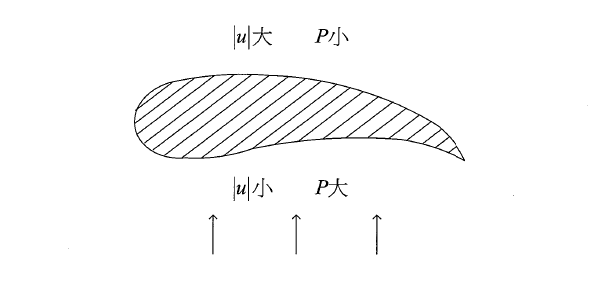
\includegraphics[width=0.5\linewidth,height=0.2\linewidth]{/ch5/fig_5_3_1.png}
	\label{img002}
	\caption{}
\end{figure}

动能 $ + $ 压力(压强) $ = $ 定数, 这式子说明了为何飞机会上升的原理.

\end{frame}

%--------------------------------------------------------------------------------------------------------------------------------------------

%----------------------------- section 4 ----------------------------------------------------------------------------------------------------

\section{\kaishu  基本电磁学理论}

%--------------------------------------------------------------------------------------------------------------------------------------------

\begin{frame}
\frametitle{\kaishu 第 \uppercase\expandafter{\romannumeral4} 节}
\begin{center}
	\Large \kaishu  基本电磁学理论
\end{center}
\end{frame}

%---------------------------------- setionc 4.1----------------------------------------------------------------------------------------------

\subsection{\kaishu 库仑定律}

%--------------------------------------------------------------------------------------------------------------------------------------------

\begin{frame}
\frametitle{ \kaishu 电场强度}

\kaishu

将电荷放在空间中时, 在其存在的位置如果有电力作用于这个电荷的空间叫做电力场, 简称电场. 放在电场内的某一点, 电量 $ q $ 的点电荷所受的电力 $ \boldsymbol{F} $ 与电量成正比, 所以

\begin{equation}
\boldsymbol{E} = \frac{\boldsymbol{F}}{q}
\label{eq5.4.1}
\end{equation}

这是那个点所定的物理量, 叫做电场强度, 意思是单位点电荷所受的作用力. 

\end{frame}

%---------------------------------------------------------------------------------------------------------------------------------------------

%--------------------------------------------------------------------------------------------------------------------------------------------

\begin{frame}
\frametitle{ \kaishu 库仑定律}

\kaishu

\small

在自然界有两种电荷, 异性相吸,同性相斥. 而电荷间作用的力和电量之乘积成正比, 与距离的平方成反比, 此定律 1776 年由英国物理学家 H. Cavendish (1731--1810) 发现, 1785 年由库仑 (Charles Augustin de Coulomb, 1736--1806) 从实验所确定. 以数学形式表示则为 

\begin{equation}
\boldsymbol{F} \propto \frac{{{q_1}{q_2}}}{{{r^2}}},\;\boldsymbol{F} = k\frac{{{q_1}{q_2}}}{{{r^2}}}
\label{eq5.4.2}
\end{equation}

此式称库仑定律. $ k $ 为一常数, 其值与所用的单位有关. 由 \ref{eq5.4.2} 可得电场

\begin{equation}
\boldsymbol{E}\left( \boldsymbol{x} \right) = \frac{q}{{{{\left| \boldsymbol{x} \right|}^2}}}\frac{\boldsymbol{x}}{{\left| \boldsymbol{x}x \right|}} = q\frac{\boldsymbol{x}}{{{{\left| \boldsymbol{x} \right|}^3}}}
\label{eq5.4.3}
\end{equation}

如果有不同的点电荷, 则利用重叠原理(线性)将各点都加起来

\begin{equation}
\boldsymbol{E}\left( \boldsymbol{x} \right) = \sum\limits_i {{q_i}\frac{{\boldsymbol{x} - {\boldsymbol{x}_i}}}{{{{\left| {\boldsymbol{x} - {\boldsymbol{x}_i}} \right|}^3}}}} 
\label{eq5.4.4}
\end{equation}

\end{frame}

%---------------------------------------------------------------------------------------------------------------------------------------------

\begin{frame}
\frametitle{\kaishu 库仑定律}

\kaishu

假设电荷分布(charge distribution) 是连续的, 则 \ref{eq5.4.4} 可写为积分形式

\vspace{0.75cm }

\begin{equation}
\boldsymbol{E}\left( \boldsymbol{x} \right) = \iiint {\rho \left( \boldsymbol{y} \right)\frac{{\boldsymbol{x} - \boldsymbol{y}}}{{{{\left| {\boldsymbol{x} - \boldsymbol{y}} \right|}^3}}}d\boldsymbol{y}}
\label{eq5.4.5}
\end{equation}

\vspace{0.75cm }

这可以视为广义库伦定律或积分形式的库伦定律, 若 $ \rho $ 已知, 则由 \ref{eq5.4.5} 可得所有静电场的问题. 但问题是大部分情形只有一部分的电荷分布为已知, 因此借助于微分方程乃是必须的. 由  Helmholtz 定理 \ref{thm5.3.6} 我们仅需知道电场 $ \boldsymbol{E} $ 的散度(divergence) 与旋度(curl). 

\end{frame}

%---------------------------------------------------------------------------------------------------------------------------------------------

\begin{frame}
\frametitle{\kaishu 库仑定律}

\kaishu

\small 

 利用关系式 $\nabla \frac{1}{{\left| {\boldsymbol{x} - \boldsymbol{y}} \right|}} =  - \frac{{\boldsymbol{x} - \boldsymbol{y}}}{{{{\left| {\boldsymbol{x} - \boldsymbol{y}} \right|}^3}}}$, 库伦定律 \ref{eq5.4.5} 可改写为
\begin{equation}
\boldsymbol{E}\left( \boldsymbol{x} \right) = \iiint {\rho \left( \boldsymbol{y} \right)\frac{{\boldsymbol{x} - \boldsymbol{y}}}{{{{\left| {\boldsymbol{x} - \boldsymbol{y}} \right|}^3}}}dy} =  - \nabla \iiint {\frac{{\rho \left( \boldsymbol{y} \right)}}{{\left| {\boldsymbol{x} - \boldsymbol{y}} \right|}}d\boldsymbol{y}}
\label{eq5.4.6}
\end{equation}

这告诉我们电场 $ \boldsymbol{E} $ 可表为某个数值函数(scalar function) 的梯度(gradient), 由此自然而然可定义电位能 $ V(\boldsymbol{x}) $

\begin{equation}
V\left( \boldsymbol{x} \right) \equiv \iiint {\frac{{\rho \left( \boldsymbol{y} \right)}}{{\left| {\boldsymbol{x} - \boldsymbol{y}} \right|}}d\boldsymbol{y}}
\label{eq5.4.7}
\end{equation}

所以库伦定律就成为

\begin{equation}
\boldsymbol{E}\left( \boldsymbol{x} \right) =  - \nabla V\left( \boldsymbol{x} \right)
\label{eq5.4.8}
\end{equation}

\end{frame}


%---------------------------------------------------------------------------------------------------------------------------------------------

\begin{frame}
\frametitle{\kaishu 库仑定律}

\kaishu

\small 

利用 \ref{eq5.4.8} 可以容易计算散度(divergence) 与旋度(curl). 首先是旋度

\begin{equation}
curl \boldsymbol{E} = \nabla \times \boldsymbol{E} = - \nabla \times \nabla V =0
\label{eq5.4.9}
\end{equation}

至于散度则需要散度定理(Gauss 定理), 先看单个点电荷

\begin{equation}
\iint {\boldsymbol{E} \cdot d\boldsymbol{S}} = \iint {E\;\cos \;\theta \;dS} = \int {\frac{{q\cos \;\theta }}{{{r^2}}}dS}  = 4\pi q
\label{eq5.4.10}
\end{equation}

若是电荷分布是连续则 \ref{eq5.4.10} 成为

\begin{equation}
\iint {\boldsymbol{E} \cdot d\boldsymbol{S}} = 4\pi \iiint {\rho \left( \boldsymbol{x} \right)d\boldsymbol{x}}
\label{eq5.4.11}
\end{equation}

\end{frame}

%---------------------------------------------------------------------------------------------------------------------------------------------

\begin{frame}
\frametitle{\kaishu 库仑定律}

\kaishu

\small 

由 Gauss 定理

\begin{equation}
\iint {\boldsymbol{E} \cdot d\boldsymbol{S}} = \iiint {div\;\boldsymbol{E}d\boldsymbol{x}} = \iiint {\nabla  \cdot \boldsymbol{E}d\boldsymbol{x}}
\label{eq5.4.12}
\end{equation}

所以

\begin{equation}
\iiint {div\;\boldsymbol{E}d\boldsymbol{x}} = 4\pi \iiint {\rho \left( \boldsymbol{x} \right)d\boldsymbol{x}}
\label{eq5.4.13}
\end{equation}

因此可得微分形式的库伦定律

\begin{equation}
div\;\boldsymbol{E}\; = \;4\pi \rho \quad (\text{\kaishu 库仑定律})
\label{eq5.4.14}
\end{equation}

\end{frame}


%---------------------------------------------------------------------------------------------------------------------------------------------

%---------------------------------------------------------------------------------------------------------------------------------------------

\begin{frame}
\frametitle{\kaishu 库仑定律之本质}

\kaishu

库伦定律就是电学的高斯定律, 我们可以理解为有电荷 $ \rho $ 才会产生电场 $ E $. 为了方便将 \ref{eq5.4.9}, \ref{eq5.4.14} 合并

\begin{equation}
\left\{ {\begin{matrix}
	{div\;\boldsymbol{E}\; = 4\pi \rho }  \\ 
	{\nabla  \times \boldsymbol{E} = \boldsymbol{0}}  \\ 
	\end{matrix}} \right.
\notag 
\end{equation}

借由电位能 $ V(\boldsymbol{E} = - \nabla V) $ 则上式成为 Poisson 方程

\begin{equation}
\Delta V =  - 4\pi \rho 
\label{eq5.4.15}
\end{equation}

\end{frame}

%---------------------------------------------------------------------------------------------------------------------------------------------

%---------------------------------- setionc 4.2------------------------------------------------------------------------------------------------

\subsection{\kaishu 安培定律}

%----------------------------------------------------------------------------------------------------------------------------------------------

\begin{frame}
\frametitle{ \kaishu 第 \uppercase\expandafter{\romannumeral4}.2 节 }
\begin{center}
	\Large \kaishu  安培定律
\end{center}
\end{frame}

%-----------------------------------------------------------------------------------------------------------------------------------------------

\begin{frame}
\frametitle{\kaishu 安培定律}
\kaishu

\small 

稳定电流通过线圈而产生的磁场是可测量的. 静磁场在任意围道(contour)的线积分(line integral)与电流成正比而与围道无关, 这就是安培定律(Ampere's law):

\begin{equation}
\oint {\boldsymbol{B} \cdot d\boldsymbol{r}}  = \frac{{4\pi }}{c}\boldsymbol{I}
\label{eq5.4.16}
\end{equation}

其中比例常数 $\frac{{4\pi }}{c}$($ c $: 光速) 是由实验而得. 我们仍然仿电场计算磁场 $ \boldsymbol{B} $ 的散度与旋度. 由于不可能创造孤立磁极(magnetic monopoles), 因此

\begin{equation}
div \boldsymbol{B} = \nabla \cdot \boldsymbol{B} = 0
\label{eq5.4.17}
\end{equation}

散度是测量场源的局部密度变化, 而由磁场的特性可知无论区域大小如何, 磁极总是有相同的北极(N)与南极(S), 故 $ div \boldsymbol{B} = \nabla \cdot \boldsymbol{B} = 0 $.


\end{frame}

%-----------------------------------------------------------------------------------------------------------------------------------------------

\begin{frame}
\frametitle{\kaishu 安培定律}

\kaishu

\small

至于旋度则可透过安培定律而来

\begin{equation}
\oint {\boldsymbol{B} \cdot d\boldsymbol{r}}  = \frac{{4\pi }}{c}I = \frac{{4\pi }}{c}\iint {\boldsymbol{J} \cdot d\boldsymbol{S}}
\label{eq5.4.18}
\end{equation}

其中 $ \boldsymbol{J} $ 是电流密度(current density), 由 Stokes 定理

\begin{equation}
\oint {\boldsymbol{B} \cdot d\boldsymbol{r}}  = \iint {\nabla  \times \boldsymbol{B} \cdot d\boldsymbol{S}}
\label{eq5.4.19}
\end{equation}

所以 \ref{eq5.4.18} 化为

\begin{equation}
\iint {\nabla  \times \boldsymbol{B} \cdot d\boldsymbol{S}} = \frac{{4\pi }}{c}\iint {\boldsymbol{J} \cdot d\boldsymbol{S}}
\notag 
\end{equation}

因此微分形式的安培定律

\begin{equation}
curl\;\boldsymbol{B} = \nabla  \times \boldsymbol{B} = \frac{{4\pi }}{c}\boldsymbol{J}, \quad  (\text{\kaishu 安培定律})
\label{eq5.4.20}
\end{equation}

\end{frame}

%-----------------------------------------------------------------------------------------------------------------------------------------------

%-----------------------------------------------------------------------------------------------------------------------------------------------

\begin{frame}
\frametitle{\kaishu 安培定律之本质}

\kaishu  


\ref{eq5.4.17}, \ref{eq5.4.20} 就是静磁场所遵循的微分方程

\begin{equation}
\nabla  \times \boldsymbol{B} = \frac{{4\pi }}{c}\boldsymbol{J},\;\;\;\nabla  \cdot \boldsymbol{B} = 0
\label{eq5.4.21}
\end{equation}

安培定律是磁学的高斯定律, 所谓静电场或静磁场之值不随时间而变化

\begin{equation}
\frac{{d{\boldsymbol{E}}}}{{dt}} = \mathop {\boldsymbol{E}}\limits^ \cdot   = \frac{{d{\boldsymbol{B}}}}{{dt}} = \mathop {\boldsymbol{B}}\limits^ \cdot   = \boldsymbol{0}.
\notag 
\end{equation}

\end{frame}


%---------------------------------- setionc 4.3-------------------------------------------------------------------------------------------------

\subsection{\kaishu 法拉第定律}

%-----------------------------------------------------------------------------------------------------------------------------------------------

\begin{frame}
\frametitle{\kaishu  第 \uppercase\expandafter{\romannumeral4}.3 节}
\begin{center}
	\Large \kaishu  法拉第定律
\end{center}

\end{frame}

%------------------------------------------------------------------------------------------------------------------------------------------------

\begin{frame}
\frametitle{\kaishu 法拉第定律}

\kaishu

\small

电场与磁场的关系是透过法拉第定律(电动势等于穿过导电电路的磁通量的变化率)来联系

\begin{equation}
\oint_C {\boldsymbol{E} \cdot d\boldsymbol{r}}  =  - \frac{\partial }{{\partial t}}\frac{1}{c}\iint_S {\boldsymbol{B} \cdot d\boldsymbol{S}},\;\;\;C = \partial S
\label{eq5.4.22}
\end{equation}

由 Stokes 定理

\begin{equation}
\oint_C {\boldsymbol{E} \cdot d\boldsymbol{r}}  = \iint_S {\nabla  \times \boldsymbol{E} \cdot d\boldsymbol{S}} =  - {\partial _t}\iint_S {\frac{1}{c}\boldsymbol{B} \cdot d\boldsymbol{S}}
\label{eq5.4.23}
\end{equation}

因此

\begin{equation}
\nabla  \times \boldsymbol{E} =  - \frac{1}{c}{\partial _t}\boldsymbol{B}
\label{eq5.4.24}
\end{equation}

此时描写电磁,磁场的方程如下

\begin{equation}
\left\{ {\begin{matrix}
	{\nabla  \times \boldsymbol{E} =  - \frac{1}{c}{\partial _t}\boldsymbol{B},}  \\ 
	{\nabla  \cdot \boldsymbol{E} = 4\pi \rho ,}  \\ 
	\end{matrix} } \right. \quad \begin{matrix}
{\nabla  \times \boldsymbol{B} = \frac{{4\pi }}{c}\boldsymbol{J}}  \\ 
{\nabla  \cdot \boldsymbol{B} = 0}  \\ 
\end{matrix} 
\label{eq5.4.25}
\end{equation}

这是静电场与静磁场之推广. 

\end{frame}

%---------------------------------- setionc 4.4-------------------------------------------------------------------------------------------------

\subsection{\kaishu 位移电流与 Maxwell 方程}

%-----------------------------------------------------------------------------------------------------------------------------------------------

\begin{frame}
\frametitle{ 第 \kaishu \uppercase\expandafter{\romannumeral4}.4 节 }
\begin{center}
	\Large \kaishu  位移电流与 Maxwell 方程
\end{center}

\end{frame}

%--------------------------------------------------------------------------------------------------------------------------------------------------

\begin{frame}
\frametitle{\kaishu 位移电流与 Maxwell 方程}

\kaishu

\small

物理学家的基本定律说到电荷是不可毁灭的, 它永远不会消失也不会被创造出来. 1860 年前后, Maxwell 发现 \ref{eq5.4.25} 这组方程式还缺少某些重要的东西. ({\color{blue} 实际上这组方程式最大的缺陷是违反电荷守恒律(conservation law of charge)}). 为此我们需要由电荷守恒律导出连续性方程(equation of continuity). 由散度定理

\begin{equation}
\iiint_\Omega  {div\;\boldsymbol{J}d\boldsymbol{x}\; = \;\iint_{\partial \Omega } {\boldsymbol{J} \cdot d\boldsymbol{S}}}
\notag 
\end{equation}

右式这个曲面积分的物理意义代表全部电流(current)流入或流出曲面 $ {\partial \Omega } $ 的量即通量(flux), 但由电荷守恒律知通量等于整个体积 $ \Omega $ 内质量的改变量

\begin{equation}
\iiint_\Omega  {div \ \boldsymbol{J}d\boldsymbol{x} = \iint_{\partial \Omega } {\boldsymbol{J} \cdot d\boldsymbol{S}}} =  - \frac{\partial }{{\partial t}}\iiint_\Omega  {\rho d\boldsymbol{x}} =  - \iiint_\Omega  {\frac{\partial }{{\partial t}}\rho d\boldsymbol{x}}
\label{eq5.4.26}
\end{equation}

因为对任意的 $ \Omega $ 上式皆成立所以 $ \rho, \boldsymbol{J} $ 满足连续性方程

\begin{equation}
\frac{{\partial \rho }}{{\partial t}} + div \ \boldsymbol{J} = \boldsymbol{0}
\label{eq5.4.27}
\end{equation}

\end{frame}

%--------------------------------------------------------------------------------------------------------------------------------------------------

\begin{frame}
\frametitle{\kaishu 位移电流与 Maxwell 方程}

\kaishu

\small

另一方面, 由安培定律 \ref{eq5.4.20} 两边取旋度得

\begin{equation}
div\;\boldsymbol{J}\; = \frac{c}{{4\pi }}div\left( {\nabla  \times \boldsymbol{B}} \right) = \boldsymbol{0}
\label{eq5.4.28}
\end{equation}

比较连续方程

\begin{equation}
\frac{c}{{4\pi }}div\left( {\nabla  \times \boldsymbol{B}} \right) = 0 = \frac{\partial }{{\partial t}}\rho  + div\;\boldsymbol{J}
\notag 
\end{equation}

但 $\rho  = \frac{1}{{4\pi }}\nabla  \cdot \boldsymbol{E}$ (假设静电场方程式成立), 则

\begin{equation}
\frac{c}{{4\pi }}\nabla  \cdot \left( {\nabla  \times \boldsymbol{B}} \right) = \nabla  \cdot \boldsymbol{J} + \frac{1}{{4\pi }}\nabla  \cdot {\partial _t}\boldsymbol{E}
\label{eq5.4.29}
\end{equation}

所以 $ \boldsymbol{B} $ 之旋度 $ curl \boldsymbol{B} = \nabla \times \boldsymbol{B} $ 满足的方程式为

\begin{equation}
\nabla  \times \boldsymbol{B} = \frac{{4\pi }}{c}\boldsymbol{J} + \frac{1}{c}{\partial _t}\boldsymbol{E}
\label{eq5.4.30}
\end{equation}

\end{frame}

%--------------------------------------------------------------------------------------------------------------------------------------------------

\begin{frame}
\frametitle{\kaishu 位移电流与 Maxwell 方程}

\kaishu

\small

将 \ref{eq5.4.25} 式重新改写为

\begin{equation}
\left\{ {\begin{matrix}
	{\nabla  \times E =  - \frac{1}{c}{\partial _t}B}  \\ 
	{\nabla  \times B = \frac{{4\pi }}{c}J + \frac{1}{c}{\partial _t}E}  \\ 
	{\nabla  \cdot E = 4\pi \rho }  \\ 
	{\nabla  \cdot B = 0}  \\ 
	\end{matrix} } \right. \quad \begin{matrix}
{\text{\kaishu 法拉第定律}}  \\ 
{\text{\kaishu 安培定律, 电荷守恒}}  \\ 
{\text{\kaishu 库仑定律}}  \\ 
{} \\ 
\end{matrix} 
\label{eq5.4.31}
\end{equation}

借着这个附加项, $\frac{{4\pi }}{c}\boldsymbol{J}$ 即所谓的位移电流来补充, 就可以克服对 \ref{eq5.4.25} 这些方程式进行数学变换, 得出一种与 Maxwell 方程系得其他公式矛盾得关系式. 因此, Maxwell 就从法拉第得解释者成为有独创性得学者. 这四个方程式就称为 Maxwell 方程(在真空), 是电磁学最基本的微分方程.

\end{frame}

%--------------------------------------------------------------------------------------------------------------------------------------------------

\begin{frame}
\frametitle{\kaishu 位移电流与 Maxwell 方程}

\kaishu

\small

由 Maxwell 方程 \ref{eq5.4.31} 直接可得的推论就是电场 $ \boldsymbol{E} $ 与磁场 $ \boldsymbol{B} $ 都满足波动方程(wave equation), 对任意的向量 $ \boldsymbol{F} $, 下式成立

\begin{equation}
\Delta \boldsymbol{F} =  - \nabla  \times \left( {\nabla  \times \boldsymbol{F}} \right) + \nabla \left( {\nabla  \cdot \boldsymbol{F}} \right)
\label{eq5.4.32}
\end{equation}

以三度空间来说

\begin{equation}
\Delta \boldsymbol{E} = {\left( {\Delta {F_1},\Delta {F_2},\Delta {F_3}} \right)^t}
\notag 
\end{equation}

向量场 $ \boldsymbol{F} $ 分布以电场 $ \boldsymbol{E} $ 与磁场 $ \boldsymbol{B} $ 代入并利用 Maxwell 方程

\begin{equation}
\Delta \boldsymbol{E} =  - \nabla  \times \left( { - \frac{1}{c}\frac{{\partial \boldsymbol{B}}}{{\partial t}}} \right) + 4\pi \nabla \rho  = \frac{1}{{{c^2}}}\frac{{{\partial ^2}\boldsymbol{E}}}{{\partial {t^2}}} + \frac{{4\pi }}{{{c^2}}}\frac{{\partial \boldsymbol{J}}}{{\partial t}} + 4\pi \nabla \rho 
\label{eq5.4.33}
\end{equation}

\begin{equation}
\Delta \boldsymbol{B} =  - \nabla  \times \left( { - \frac{1}{c}\frac{{\partial \boldsymbol{E}}}{{\partial t}} + \frac{{4\pi }}{c}\boldsymbol{J}} \right) = \frac{1}{{{c^2}}}\frac{{{\partial ^2}\boldsymbol{B}}}{{\partial {t^2}}} - \frac{{4\pi }}{{{c^2}}}\nabla  \times \boldsymbol{J}
\label{eq5.4.34}
\end{equation}

 

\end{frame}

%--------------------------------------------------------------------------------------------------------------------------------------------------

\begin{frame}
\frametitle{\kaishu 位移电流与 Maxwell 方程}

\kaishu

\small 

换句话说, $ \boldsymbol{E},\boldsymbol{B} $ 满足非齐次波动方程

\begin{equation}
{\boldsymbol{E}_{tt}} - {c^2}\Delta \boldsymbol{E} =  - 4\pi \left( {{c^2}\nabla \rho  + {\boldsymbol{J}_t}} \right)
\label{eq5.4.35}
\end{equation}

\begin{equation}
{\boldsymbol{B}_{tt}} - {c^2}\Delta \boldsymbol{B} = 4\pi c\left( {\nabla  \times \boldsymbol{J}} \right)
\label{eq5.4.36}
\end{equation}

如果考虑的区域没有电荷或电流, 则 $ \boldsymbol{E},\boldsymbol{B} $ 满足齐次波动方程.

\begin{equation}
{\boldsymbol{E}_{tt}} - {c^2}\Delta \boldsymbol{E} = {\boldsymbol{B}_{tt}} - {c^2}\Delta \boldsymbol{B} = 0
\label{eq5.4.37}
\end{equation}

\ref{eq5.4.35},\ref{eq5.4.36} 还告诉我们电场,磁场是以光速 $ c $ 传播, 也因此我们习惯通称为电磁波.

\end{frame}

%---------------------------------------------------------------- section 5 ------------------------------------------------------------------------

\section{\kaishu 参考文献}

%---------------------------------------------------------------------------------------------------------------------------------------------------

\begin{frame}
\frametitle{\kaishu \uppercase\expandafter{\romannumeral5} 参考文献}
\footnotesize{
	\begin{thebibliography}{99} % Beamer does not support BibTeX so references must be inserted manually as below
		\bibitem[1]{p1} \kaishu 林琦焜 (2007),  \kaishu <<向量分析>>, 沧海书局, 2007.
	\end{thebibliography}

	\vspace{1cm}
	
	\begin{thebibliography}{99} % Beamer does not support BibTeX so references must be inserted manually as below
		\bibitem[2]{p2} \kaishu 费曼,莱顿,桑兹著; 李洪芳,王子辅,钟万蘅译 (2020),  \kaishu <<费曼物理学讲义>>, 上海科学技术出版社, 2020.
	\end{thebibliography}
	
}
\end{frame}

%----------------------------------------------------------------------------------------------------------------------------------------------------

\begin{frame}
\frametitle{\kaishu 最后了}
\begin{center}
	{\Huge Thank you!}
	
	\vspace{1cm}
	
	{\Huge Any comments or questions?}
	
	\vspace{2.25cm}	
	
  {\tiny Welcome to visit my personal homepage}	
  	
  {	\tiny {\color{blue} \url{https://zhims.github.io/}}}
\end{center}
\end{frame}

%-------------------------------------------------------------------------------------------------------------------------------------------------

\end{document} 